
\documentclass{article}
\usepackage{pgfplots}
\pgfplotsset{compat=1.18}
\usepackage{tikz}
\usepackage{xcolor}
\usepackage{amsmath}
\usepackage{PRIMEarxiv}
\usepackage[utf8]{inputenc}
\usepackage[T1]{fontenc}
\usepackage{hyperref}
\usepackage{url}
\usepackage{booktabs}
\usepackage{amsfonts}
\usepackage{nicefrac}
\usepackage{microtype}
\usepackage{lipsum}
\usepackage{multirow}
\usepackage{graphicx}
\usepackage{float}
\usepackage{caption}
\usepackage{pifont}
\newcommand{\cmark}{\ding{51}}
\newcommand{\xmark}{\ding{55}}
\graphicspath{{media/}}
\definecolor{archblue}{RGB}{31,78,121}
\definecolor{archblue2}{RGB}{91,138,179}
\definecolor{fidelitygold}{RGB}{160,100,0}
\definecolor{gridgray}{RGB}{225,225,225}
\captionsetup[table]{skip=5pt}

\title{EMA-Gated Temporal Sequence Compression in Vision Transformers}

\author{Yannick Schmitt \\ 
\texttt{ynnk.schmitt@gmail.com} \\
\vspace{4pt} 
\href{https://doi.org/10.5281/zenodo.19337577}{DOI: 10.5281/zenodo.19337577}}
\begin{document}
\maketitle

\begin{abstract}
We introduce \textbf{NeuroFlow}, a dynamic routing framework for Vision
Transformer video inference that exploits temporal redundancy by tracking
per-patch semantic surprise via an Exponential Moving Average~(EMA) of
patch-level embeddings. The central contribution is the
\textbf{Dual-Memory Reconstruction Protocol} (Architecture~C): a
\emph{training-free} inference engine that combines a Retinal Gate
(Layer~0 EMA, eliminating stationary tokens before the encoder) with a
Cortical Cache (persistent Layer~12 encoder output buffer, supplying the
full $N$-token K-V set to the pooling head from cache). Without any
fine-tuning or weight modification, Architecture~C achieves
\textbf{71.55\% UCF-101 zero-shot top-1 accuracy at 84.0\% token
sparsity} on SigLIP base-patch16-224, retaining 92.4\% of dense
accuracy. The design is grounded in two empirical laws: the
\emph{Saturation Law} (accuracy gap is invariant to skip rate above 65\%;
operate at MaxSparse) and the \emph{Degradation Law} (gap $\approx
4.5 + 0.7\cdot\max(0, \sigma-1.0)$\,pp, where $\sigma$ is the
positional-embedding stretch factor). Architecture~C is constrained to
resolutions $\leq$448p by the PE interpolation boundary; it targets
edge inference where the absence of fine-tuning outweighs reduced
speedup.

For applications requiring near-2K throughput, \textbf{Architecture~B}
physically eliminates stationary tokens before the encoder, reducing
1792p SigLIP~2 inference from 678\,ms to 11.9\,ms---a
$\mathbf{55.80\times}$ wall-clock speedup at 97.37\% embedding fidelity
with sparse manifold distillation. The primary obstacle to naive sparse
fidelity is the MAP head's K-V pooling concentration, not the encoder: a
finding confirmed via direct entropy measurement across two SigLIP
generations. Architecture~A (late-layer MLP gating) is bounded by
Amdahl's Law at $1.17\times$ maximum speedup at 1792p and is
characterised as the correct design for $\mathcal{O}(N)$-attention
architectures only.

A cross-domain ablation on Phi-3-mini characterises the architectural
boundary that determines when the similarity-gating principle transfers
to autoregressive language models. The \emph{PPL-Drift Dissociation}
(high token drift coexists with $\Delta\mathrm{PPL} < 0.04$ because bypass
navigates equiprobable semantic paths) and the \emph{Entropy-Bypass
Correlation} (code generation: 0\% drift at 21\% bypass; prose: 83\%
drift at any bypass rate) define the deployment safety envelope. Current
hardware is memory-bandwidth bound at all practical batch sizes
($1.000\times$ wall-clock speedup); the path to latency gains requires
MLP-only bypass or kernel-level weight-skip support.
\end{abstract}

\keywords{Vision Transformers \and Temporal Sequence Compression \and
Gating Mechanisms \and Exponential Moving Average (EMA) \and Efficient
Deep Learning}


\begin{figure}[t]
\centering
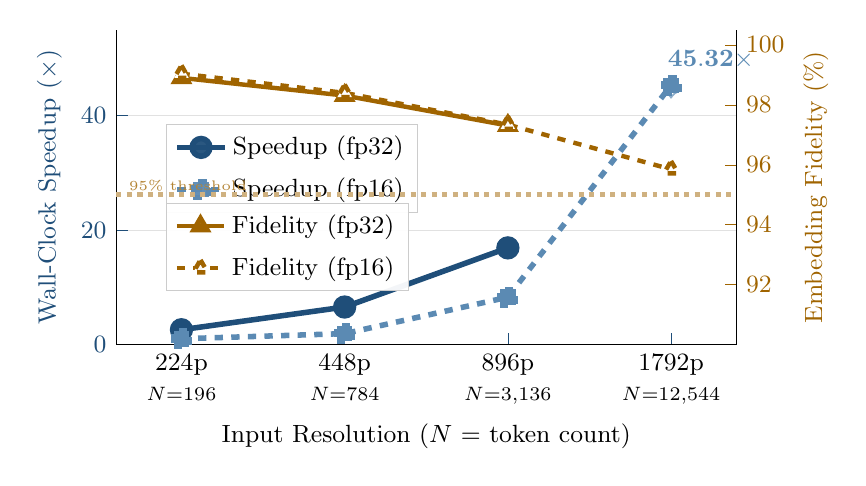
\begin{tikzpicture}
\begin{axis}[
    name=mainax,
    width=0.78\textwidth,
    height=0.46\textwidth,
    xlabel={Input Resolution ($N$ = token count)},
    ylabel={Wall-Clock Speedup ($\times$)},
    xtick={1,2,3,4},
    xticklabels={
        {224p \\ \scriptsize$N{=}196$},
        {448p \\ \scriptsize$N{=}784$},
        {896p \\ \scriptsize$N{=}3{,}136$},
        {1792p \\ \scriptsize$N{=}12{,}544$}
    },
    xticklabel style={align=center, font=\small},
    yticklabel style={font=\small, text=archblue},
    ylabel style={font=\small, text=archblue},
    xlabel style={font=\small},
    ymin=0, ymax=55,
    xmin=0.6, xmax=4.4,
    ymajorgrids=true,
    grid style={gridgray, very thin},
    axis y line*=left,
    axis x line*=bottom,
    tick style={archblue},
    legend style={
        at={(0.08,0.70)},
        anchor=north west,
        font=\small,
        draw=gray!40,
        fill=white,
        fill opacity=0.95,
        text opacity=1,
        row sep=3pt,
        /tikz/every even column/.append style={column sep=0.4em}
    },
    legend cell align=left,
    clip=false,
]
\addplot[color=archblue, line width=2pt, mark=*, mark size=3.2pt,
    mark options={fill=archblue, draw=archblue}]
    coordinates { (1,2.60) (2,6.57) (3,16.91) };
\addlegendentry{Speedup (fp32)};
\addplot[color=archblue2, line width=2pt, dashed, mark=square*, mark size=2.8pt,
    mark options={fill=archblue2, draw=archblue2}]
    coordinates { (1,1.02) (2,1.92) (3,8.29) (4,45.32) };
\addlegendentry{Speedup (fp16)};
\node[font=\small\bfseries, text=archblue2, anchor=south west]
    at (axis cs:3.92, 46.5) {$\mathbf{45.32\times}$};
\draw[->, thick, archblue2!70]
    (axis cs:4.0, 45.5) -- (axis cs:4.0, 43.0);
\end{axis}
\begin{axis}[
    at={(mainax.south east)},
    anchor=south east,
    width=0.78\textwidth,
    height=0.46\textwidth,
    xmin=0.6, xmax=4.4,
    ymin=90, ymax=100.5,
    ylabel={Embedding Fidelity (\%)},
    ylabel style={font=\small, text=fidelitygold},
    yticklabel style={font=\small, text=fidelitygold},
    tick style={fidelitygold},
    axis y line*=right,
    axis x line=none,
    xtick=\empty,
    ytick={92,94,96,98,100},
    legend style={
        at={(0.08,0.45)}, anchor=north west, font=\small,
        draw=gray!40, fill=white, fill opacity=0.95,
        text opacity=1, row sep=3pt,
    },
    legend cell align=left,
    clip=false,
]
\addplot[color=fidelitygold, line width=1.6pt, mark=triangle*, mark size=3pt,
    mark options={fill=fidelitygold, draw=fidelitygold}]
    coordinates { (1,98.90) (2,98.31) (3,97.31) };
\addlegendentry{Fidelity (fp32)};
\addplot[color=fidelitygold, line width=1.6pt, dashed, mark=triangle*,
    mark size=3pt, mark options={fill=white, draw=fidelitygold}]
    coordinates { (1,99.04) (2,98.40) (3,97.34) (4,95.85) };
\addlegendentry{Fidelity (fp16)};
\addplot[color=fidelitygold!50, line width=1.8pt, dotted, domain=0.6:4.4] {95};
\node[font=\tiny, text=fidelitygold!80, anchor=west]
    at (axis cs:0.62, 95.3) {95\% threshold};
\end{axis}
\end{tikzpicture}
\caption{%
    \textbf{Architecture~B fine-tuned wall-clock speedup and embedding
    fidelity vs.\ input resolution} (SigLIP base-patch16-224, GPU, sparse
    manifold distillation).
    Left axis (blue): wall-clock speedup over dense baseline.
    Right axis (gold): cosine similarity to dense output.
    Speedup scales superlinearly with resolution as the
    $\mathcal{O}(N_{\mathrm{active}}^2)$ attention cost shrinks with token
    skip rate~$\rho$. At 1792p ($N{=}12{,}544$, $\rho{=}92.8\%$),
    inference is reduced from 582\,ms to 12.85\,ms\,---\,$\mathbf{45.32\times}$
    wall-clock speedup (fp16)\,---\,at 95.85\% embedding fidelity and
    100\% semantic top-3 accuracy.
    Dashed: fp16\,;\ solid: fp32. Dotted gold line: 95\% fidelity threshold.%
}
\label{fig:teaser}
\end{figure}

\section{Introduction}\label{sec:introduction}

The deployment of Vision Transformers for real-time video understanding
is constrained by a fundamental architectural mismatch: the
self-attention mechanism scales quadratically with the number of input
tokens, $\mathcal{O}(N^2)$, while natural video is dominated by temporal
continuity. A frame from a traffic camera at $1792{\times}1792$ pixels
produces $N=12{,}544$ patch tokens, the overwhelming majority of which
are spatially and semantically identical to the preceding frame. Standard
inference pipelines compute dense attention over all tokens at every
frame---recalculating the latent representations of static asphalt,
empty sky, and stationary infrastructure at full cost.

The correct response to this mismatch is not to compress the model but
to \emph{not compute what has not changed}. We introduce \textbf{NeuroFlow},
a gate that tracks per-patch semantic surprise via an Exponential Moving
Average (EMA) of patch-level embeddings and routes computation
proportionally to surprise. The central insight of this work, arrived at
through a sequence of failed approaches, is that sparse inference is
best framed as a \emph{memory management problem}, not a learning problem:
the encoder is a computation-heavy semantic generator, and the pooling
head is a memory-hungry integrator. Decoupling these two roles---using
the encoder only for semantically changed patches and serving the pooling
head from a persistent cache of prior representations---produces a system
that is simultaneously fast and generalisation-preserving.

\paragraph{The Dual-Memory Reconstruction Protocol (Architecture C).}
The central contribution is Architecture~C, a training-free inference
engine combining a Retinal Gate (Layer~0 EMA, eliminating stationary
tokens before the encoder) with a Cortical Cache (a persistent buffer of
Layer~12 encoder outputs that reconstructs the full $N$-token
representation for the pooling head without re-encoding). Without any
fine-tuning, Architecture~C achieves \textbf{71.55\% UCF-101 zero-shot
top-1 accuracy at 84.0\% token sparsity}, retaining 92.4\% of dense
accuracy. The design generalises across video domains (51--97\% skip
rates on first-person drone and racing footage) and its behaviour is now
characterised by four empirical laws---Degradation, Saturation, Capacity,
and Spatial Displacement---each with actionable deployment implications.

Architecture~C's validity rests on a structural property: Layer~12
representations of stationary patches maintain $0.83$ cosine stability
across frames, sufficient for the pooling head's softmax distribution to
recover its original shape from one-frame-stale cache vectors. This is
substantially better than the $\leq 0.60$ cosine ceiling achievable by
any linear Layer~0-to-Layer~12 projection (the Representation Gap),
which invalidates hallucinative reconstruction and motivates identity
caching as the only sound design.

\paragraph{Why earlier approaches failed.}
Two alternative placements of the gate were evaluated before Architecture~C.
Architecture~A inserts the gate between the attention and MLP sub-layers,
saving $\mathcal{O}(N)$ MLP compute while preserving the full
$\mathcal{O}(N^2)$ attention matrix. At 1792p, attention consumes
$\sim$85\% of frame time, bounding Architecture~A's maximum speedup at
$\mathbf{1.17\times}$ by Amdahl's Law regardless of skip rate. It is the
correct design for $\mathcal{O}(N)$-attention architectures (Swin,
linear-attention variants) but not for standard ViTs at high resolution.

Architecture~B moves the gate to Layer~0 and physically eliminates
inactive tokens before the encoder, reducing attention cost to
$\mathcal{O}(N_{\text{active}}^2)$ and achieving $\mathbf{55.80\times}$
wall-clock speedup at 1792p on SigLIP~2. Applied to an unmodified model,
Architecture~B produces systematic embedding collapse (45--76\% cosine
similarity) because the MAP head's cross-attention pooling fails when
its K-V set contracts to $\leq$6 tokens. Sparse manifold distillation
resolves this within the fine-tuned domain, but at the cost of
catastrophic forgetting: 2.40\% UCF-101 zero-shot top-1 accuracy
post-fine-tuning versus 77.40\% for the base model. This collapse arises
because the fine-tuning objective optimises embedding direction (cosine)
but not semantic scope.

Architecture~C resolves this tension entirely by supplying the MAP head
with a structurally complete K-V set at every frame---active tokens from
the encoder, inactive tokens from the Cortical Cache---without modifying
any parameters. Architecture~C is constrained to resolutions $\leq$448p
by the positional-embedding interpolation boundary, positioning it as
the correct design for edge inference and CPU-constrained pipelines where
zero fine-tuning outweighs reduced speedup.

\paragraph{Contributions.}
\begin{itemize}
  \item \textbf{Architecture~C: Dual-Memory Reconstruction Protocol.}
    A training-free inference engine that decouples encoder sparsity from
    pooling-head completeness via the Cortical Cache. Four empirical laws
    completely characterise its deployment behaviour; the Saturation Law
    provides the operational conclusion: deploy at MaxSparse.
  \item \textbf{Architecture~B wall-clock acceleration.}
    $55.80\times$ wall-clock speedup at 1792p on SigLIP~2 after sparse
    manifold distillation; $45.32\times$ on SigLIP~v1. The MAP head's
    K-V pooling concentration is identified as the primary fidelity
    obstacle---distinct from encoder robustness---and is characterised
    empirically across two SigLIP generations.
  \item \textbf{Architecture~A: Amdahl ceiling and O$(N)$-attention target.}
    Late-layer MLP gating is bounded at $1.17\times$ at high resolution.
    The gate design is correct; the constraint is architectural. A fused
    CUDA kernel would lower the crossover below 224p, making Architecture~A
    viable for windowed-attention and linear-attention models.
  \item \textbf{Cross-domain LLM ablation.}
    The Entropy-Bypass Correlation and PPL-Drift Dissociation characterise
    the safety envelope and architectural boundary for similarity-gated
    bypass in autoregressive language models. Wall-clock benefit is
    bandwidth-bound on current hardware; MLP-only bypass and
    self-speculative decoding are identified as the viable engineering paths.
  \item \textbf{Emergent zero-shot capabilities.}
    Motion segmentation, cluster-level semantic classification, and
    identity-preserving spatial tracking arise from the gate's spatial
    mask output without additional parameters.
\end{itemize}

\section{Related Work}\label{related-work}

\subsection{Token Pruning and Dynamic ViTs}

DynamicViT \cite{rao2021dynamicvit} introduces a learned prediction module
that determines token importance per image, dropping tokens from
intermediate layers. While effective, this approach requires training the
prediction module jointly with the backbone and operates on static images
without temporal context. ToMe \cite{bolya2023tokenmergingvitfaster}
merges similar tokens using bipartite matching rather than dropping them,
preserving more information at the cost of a larger effective sequence.
Both methods reduce theoretical FLOPs but do not guarantee wall-clock
speedup on current GPU hardware due to lack of kernel-level support for
ragged sequence lengths.

NeuroFlow's Architecture~B differs in three respects: (i)~the gating
signal is derived from temporal history via EMA, not from intra-frame
feature similarity; (ii)~tokens are physically eliminated before the
encoder, not pruned at intermediate layers; and (iii)~no learned
prediction module is added to the backbone---the gate is applied purely
to the patch embedding output.

\subsection{Efficient Attention Mechanisms}

Linear attention variants \cite{katharopoulos2020transformers,choromanski2021rethinking}
rewrite the attention kernel to reduce complexity from $\mathcal{O}(N^2)$
to $\mathcal{O}(N)$, enabling Architecture~A's MLP gating approach to scale
effectively. Windowed attention (Swin Transformer \cite{liu2021swin})
restricts attention to local windows, reducing attention cost to $\mathcal{O}(N)$
at the expense of global context. NeuroFlow's analysis identifies these
architectures as the natural target for Architecture~A: when attention is
$\mathcal{O}(N)$, gating the $\mathcal{O}(N)$ MLP produces proportional
speedups without Amdahl's ceiling.

\subsection{Temporal Redundancy in Video}

Video-specific ViT variants \cite{arnab2021vivit,bertasius2021spacetime}
extend spatial attention to the temporal dimension via factorised or joint
space-time attention. These approaches increase compute relative to
single-frame inference and do not address the redundancy problem.
Frame-skipping policies \cite{wu2019longterm} use lightweight models to
determine when a heavy model needs to re-run; NeuroFlow's EMA gate
performs an analogous function at patch granularity within a single model.

\subsection{Knowledge Distillation for Sparse Models}

Sparse manifold distillation in NeuroFlow is most closely related to
self-distillation approaches including DINO \cite{caron2021dino} and
SILC \cite{naeem2023silc}, where a student with a restricted view (local
crop or sparse token set) is trained to reproduce the global representation
of a dense teacher. The key difference is that NeuroFlow's student sees a
temporally-filtered sparse sequence rather than a spatially-cropped local
view, and the teacher is the same model architecture running in dense
mode on the same frame.

\subsection{TIPS and Masked Pre-training}

TIPS \cite{zhai2024siglip2} pre-trains SigLIP~2 with 50\% random token
masking, explicitly training the encoder to produce stable representations
under partial inputs. This is the closest prior work to our sparse sequence
setting. We evaluate the transfer of TIPS robustness to NeuroFlow's
temporally-correlated gating regime and find partial but insufficient
transfer, characterising the precise mechanism by which it falls short.

\subsection{Layer-Skipping and Early Exit in Transformers}
\label{rw:layer-skipping}

Dynamic early exit \cite{teerapittayanon2016branchynet,xin2020deebert}
and confident adaptive computation \cite{schuster2022calm} allow tokens
or sequences to exit at intermediate layers when prediction confidence
exceeds a threshold. SkipDecode \cite{del2023skipdecode} extends this to
batched autoregressive decoding. LayerSkip \cite{elbayad2024layerskip}
explicitly trains models to support early exit at any layer and uses
early-exit outputs as draft tokens for speculative decoding.
These approaches require either joint training of exit classifiers or
architectural modifications. Architecture~C contributes a complementary
finding for encoder-only vision models: the relevant redundancy is
\emph{spatial} (across patches in a frame) rather than
\emph{depth}-based (across layers for a sequence), and the correct
response to redundancy is identity caching of the final-layer
representation, not early exit.

\subsection{KV-Cache Reuse and Speculative Decoding}
\label{rw:kvcache}

Speculative decoding \cite{leviathan2023speculative,chen2023speculative}
uses a small draft model to generate candidate tokens that a larger
target model verifies in parallel. Self-speculative decoding
\cite{elbayad2024layerskip} eliminates the draft model by using
early-exit paths of the target model itself. Our LLM ablation
(Section~\ref{sec:llm-ablation}) empirically demonstrates that
NeuroFlow's mid-deep bypass acts as an implicit self-drafter: the
$L_1{\to}L_{31}$ route produces fluent, grammatically valid text
($\Delta\mathrm{PPL} < 0.03$) while deviating from the dense
trajectory, precisely the acceptance-rate profile required for a
high-utility draft model.

\subsection*{Relationship to EventViT}

DVS-ViT~\cite{dvsvit2022} applies active patch selection to Vision
Transformers processing event camera data, eliminating patches whose
event activity ratio falls below a threshold before the encoder. This
shares the core architectural commitment of Architecture~B---physical
token elimination before the encoder rather than intermediate-layer
pruning---and independently validates the same finding: that ViTs are
robust to variable-length input sequences when the eliminated patches
correspond to low-information regions. The key distinction is the
activity signal: DVS-ViT operates on pixel-domain event counts from
sensor physics; NeuroFlow operates on semantic surprise in embedding
space, which is robust to photometric variation (illumination gradients,
shadows, compression artefacts) that would produce spurious activity in
the pixel domain.


\section{Architecture}\label{architecture}
\subsection{Architecture~C: The Dual-Memory Reconstruction Protocol}
\label{sec:arch-c-method}

Architecture~C is the paper's central contribution. It decouples two
distinct roles that a naive sparse encoder conflates:
(a)~\emph{the encoder}, whose job is to generate contextually enriched
Layer~12 patch representations, and (b)~\emph{the MAP head}, whose job
is to pool over a complete set of $N$ K-V pairs to produce a stable
global embedding. These two requirements are satisfied by different
sources:

\begin{itemize}
    \item \textbf{Retinal Gate (Layer~0 EMA).} The EMA surprise signal
    $s_i^t = 1 - \cos(h_i^t, E_i^{t-1})$ determines the active set
    $\mathcal{A}^t$ at each frame. Active patches (high surprise) are
    forwarded through the full encoder. Inactive patches are not.
    \item \textbf{Cortical Cache (Layer~12 Buffer).} A persistent buffer
    $\mathcal{C} \in \mathbb{R}^{N \times D}$ stores the Layer~12 encoder
    output $z_i^{t'}$ for each patch $i$, where $t'$ is the most recent
    frame at which patch $i$ was active. At every frame, the cache is
    updated only for active patches:
\end{itemize}

\begin{equation}
    \label{eq:cache-update}
    \mathcal{C}_i^t \;=\;
    \begin{cases}
        z_i^t & \text{if } i \in \mathcal{A}^t \\
        \mathcal{C}_i^{t-1} & \text{otherwise}
    \end{cases}
\end{equation}

The MAP head receives the full $N$-token sequence $\mathcal{C}^t$ at
every frame: fresh Layer~12 outputs for active patches, cached outputs
from the most recent active frame for inactive patches. No fine-tuning
is applied to the encoder or MAP head.

\textbf{Computational structure.}
The encoder processes only $N_{\text{active}} = |\mathcal{A}^t|$ tokens,
preserving the $\mathcal{O}(N_{\text{active}}^2)$ attention speedup of
Architecture~B. The MAP head runs at $\mathcal{O}(Q \cdot N)$ cost where
$Q$ is the number of learned query vectors, regardless of skip rate. At
high resolutions the MAP head cost is a small fraction of total encoder
cost and overall speedup approaches Architecture~B. At 224p the MAP head
cost is relatively larger; speedup is lower than Architecture~B but
fidelity is substantially higher without any training.

\textbf{Why this works.}
The protocol's validity rests on two empirical conditions: (1)~Layer~12
representations for stationary patches are temporally stable,
i.e.\ $\cos(z_i^t, z_i^{t-1})$ is high for patches with $s_i^t < \theta$;
and (2)~the MAP head's softmax distribution recovers its original shape
when provided a structurally complete K-V set, even if inactive token
representations are one frame stale. Both conditions are validated in
Section~\ref{sec:arch-c-stability}.

\textbf{Why projection fails.}
Section~\ref{sec:representation-gap} establishes the Representation Gap:
any linear Layer~0$\to$Layer~12 projection is structurally bounded at
$\leq 0.60$ cosine similarity. Using such projections to fill the MAP
head's K-V set introduces $\geq 40\%$ error per reconstructed token,
inducing the accuracy collapse observed under naive sparse inference.
The Cortical Cache avoids this entirely: it recycles the actual Layer~12
representation, not an approximation.

\subsection{Architecture B: Early Token Elimination}
\label{sec:arch-b}

Architecture~B moves the gate to Layer~0---the patch embedding
layer---and physically eliminates inactive tokens from the tensor before
any encoder computation. The compressed sequence $h^t[\mathcal{A}^t]$
of length $N_{\text{active}}$ is passed through all Transformer layers.
Because self-attention operates on the compressed sequence, its cost is
$\mathcal{O}(N_{\text{active}}^2)$ rather than $\mathcal{O}(N^2)$,
yielding superlinear compute reduction with skip rate
$\rho = 1 - N_{\text{active}}/N$.

Spatial ordering of active tokens is preserved by sorting $\mathcal{A}^t$
before indexing. A minimum token floor ($N_{\mathrm{floor}} = 4$) ensures
the MAP head always receives at least 4 K-V pairs. The EMA is updated
unconditionally at each frame using the full embedding $h^t$ (before
gating) so that background patches continue to be tracked even when
eliminated from the encoder pass.

Applied to an unmodified model, Architecture~B produces systematic
fidelity collapse (45--76\% cosine similarity) because the MAP head's
cross-attention pooling fails when its K-V set contracts to $\leq$6
tokens. Sparse manifold distillation (§\ref{sec:distillation}) is
required to adapt the MAP head to the sparse pooling regime.
Architecture~C bypasses this requirement entirely via the Cortical Cache
design.

\subsection{Sparse Manifold Distillation}
\label{sec:distillation}

Sparse manifold distillation fine-tunes the model to reproduce the dense
output of a frozen teacher copy when presented with a gate-filtered
sparse input sequence. The distillation objective operates on
$\ell^2$-normalised embeddings of the student (sparse) and teacher
(dense) on the unit hypersphere, combining a cosine alignment term with
a normalised MSE term. Both student and teacher are from the same model
family; cross-family distillation is avoided because SigLIP v1 and v2
embed into geometrically distinct representation spaces.

Training employs temporal video clips as the primary data modality, with
the EMA gate threshold and decay rate randomised per clip to expose the
model to the full range of sparsity regimes it will encounter at
inference. This curriculum ensures that the MAP head is trained under the
high-skip conditions that correspond to its deployment operating point.

\textbf{Limitation.}
Fine-tuning on a narrow domain with cosine distillation induces
catastrophic forgetting (UCF-101 top-1: 2.40\% post-fine-tuning vs.\
77.40\% base). The forgetting arises from narrow label distribution
during training, not from the distillation objective per se.
Remediation: diverse training data, MSE embedding preservation loss
(which jointly constrains direction and magnitude), and learning rate
$\leq 5 \times 10^{-6}$ for $\leq 3$ epochs. The distillation objective
also does not constrain embedding magnitude; for unnormalised evaluation
protocols, MSE loss should replace or supplement the cosine objective.
Architecture~C avoids all of these constraints by requiring no training.

\subsection{Architecture A: The Amdahl Ceiling}
\label{sec:arch-a}


Architecture~A inserts the NeuroFlow gate between the self-attention
and MLP sub-layers of each Transformer block. Tokens whose surprise score
falls below $\theta$ retain their keyframe-derived features rather than
updating through the MLP. The full $N$-token sequence remains present in
memory, enabling all-to-all self-attention at $\mathcal{O}(N^2)$ while
saving $\mathcal{O}(N)$ MLP compute for dormant tokens.

Architecture~A achieves 97.1\% fidelity at 81.9\% token sparsity. Its
practical limitation is the $\mathcal{O}(N^2)$ attention floor, which
renders it ineffective for wall-clock speedup on standard ViTs at high
resolution: Amdahl's Law bounds maximum speedup at $1.17\times$ at
1792p regardless of MLP skip rate (Section~\ref{sec:architecture-a-amdahls-ceiling}).
Empirical results confirm this bound (Section~\ref{sec:architecture-a-amdahls-ceiling}).

Architecture~A represents the correct design for architectures with
$\mathcal{O}(N)$ attention complexity. For Swin Transformer variants and
linear-attention models, the MLP constitutes a larger fraction of total
compute and MLP gating achieves proportional speedups without the
Amdahl ceiling. A naive variant passing stale $t-1$ features forward
without a keyframe anchor induces catastrophic fidelity collapse
(13.2--36.5\% cosine similarity) due to feature drift between temporal
manifolds; the anchor mechanism is essential.

\subsection{Architecture D: A Closed Research Direction}
\label{sec:arch-d}
\label{sec:representation-gap}


Architecture~D extends Architecture~C by running Layers~0--$K$ densely
on all $N$ tokens (providing shared context) and Layers~$K$+1--12
sparsely on the active set. The theoretical prediction was that shared
early-layer context would reduce active shift. The data refutes this
entirely.

\begin{table}[htbp]
\centering
\setlength{\tabcolsep}{4.5pt}
\renewcommand{\arraystretch}{1.12}
\begin{tabular}{lrrl}
\toprule
\textbf{Layer $K$} & \textbf{Cos$(K,12)$} & \textbf{Std}
  & \textbf{Representation Gap} \\
\midrule
Layer~0  & 0.049 & 0.008 & 95.1\% (Arch~C gate, baseline) \\
Layer~2  & 0.072 & 0.011 & 92.8\% \\
Layer~4  & 0.104 & 0.023 & 89.6\% \\
Layer~6  & 0.198 & 0.043 & 80.2\% \\
Layer~8  & 0.328 & 0.043 & 67.2\% \\
Layer~10 & 0.508 & 0.025 & 49.2\% \\
\bottomrule
\end{tabular}
\caption{Cosine similarity between Layer-$K$ and Layer-12 representations.
The gap remains above 80\% through Layer~6, closing meaningfully only
at Layers~8--10. Contextual entanglement is concentrated in the final
2--4 encoder layers, not distributed uniformly across depth.}
\label{tab:representation-gap}
\end{table}

\begin{table}[htbp]
\centering
\setlength{\tabcolsep}{4pt}
\renewcommand{\arraystretch}{1.12}
\begin{tabular}{llrrrrr}
\toprule
\textbf{Architecture} & \textbf{Config} & \textbf{T1} & \textbf{Gap}
  & \textbf{Latency} & \textbf{Speedup} & \textbf{vs.\ Arch~C} \\
\midrule
Dense   & ---         & 77.25\% & ---     & 8.27\,ms & 1.00$\times$ & --- \\
Arch~C  & $g=0, K=12$ & 73.00\% & +4.25\,pp & 6.60\,ms & 1.25$\times$ & --- \\
Arch~D  & $g=1, K=3$  & 73.00\% & +4.25\,pp & 7.81\,ms & 1.06$\times$
  & $-0.00$\,pp / $+1.21$\,ms \\
\bottomrule
\end{tabular}
\caption{Architecture~D vs.\ Architecture~C at 224p ($n=400$ clips).
The 1.21\,ms overhead of Arch-D's shared dense context pass yields zero
accuracy improvement. At 896p the overhead is $+27.4$\,ms; at 1792p it
is $+315.5$\,ms ($21\times$ slower). Architecture~D is strictly dominated
by Architecture~C at all tested resolutions: same accuracy, higher latency.}
\label{tab:arch-d-comparison}
\end{table}

The failure is explained by the Representation Gap data: cos$(K, 12)
\leq 0.20$ for $K \leq 6$, meaning shared context through the first 6
layers provides representations that differ from Layer-12 by 80\% cosine
distance. The contextual structure that determines Layer-12 representation
is established in the \emph{final} 2--4 encoder layers, not the first half.
Running structurally incomplete representations as dense context anchors
provides no meaningful reduction in active shift. Architecture~C is the
Pareto frontier of the EMA-gated Dual-Memory design space; Architecture~D
is closed as a research direction.

\subsection{Scene-Type Generalisation and Deployment Boundaries}
\label{sec:motion-generalisation}

Architecture~C accuracy degradation is not uniform across action classes.
The aggregate 4.89\,pp gap conceals a bimodal distribution spanning
from active improvement to catastrophic failure.

\textbf{Motion speed does not predict degradation.}
Optical flow magnitude (mean absolute pixel displacement per frame) is
non-predictive of the accuracy gap. The gap is highest in the low-motion
quartile (flow $\leq$ 1.23 px/frame, $+10$\,pp) and comparable in the
dynamic quartile ($>$5.03 px/frame, $+8$\,pp). Motion speed cannot serve
as a deployment suitability predictor.

\textbf{Spatial displacement of the action region predicts degradation.}
The centroid of the optical-flow-active region predicts the gap: it
increases from $+2$--$4$\,pp in the Local quartile (centroid displacement
$\leq$ 0.069 normalised units) to $+7$--$8$\,pp in the Traversal
quartile ($>$0.165). Within-class analysis confirms this is a within-class
mechanism, not a class-label confound.

\begin{table}[htbp]
\centering
\setlength{\tabcolsep}{4pt}
\renewcommand{\arraystretch}{1.12}
\begin{tabular}{lrrrrl}
\toprule
\textbf{Class} & $n$ & \textbf{Dense T1}
  & \textbf{MaxSp T1} & \textbf{Gap} & \textbf{Mechanism} \\
\midrule
Swing             & 7 & 57\%  & 14\% & +43\,pp & Arc traversal (centroid disp: 0.274) \\
YoYo              & 6 & 100\% & 67\% & +33\,pp & Oscillating object: cache cycles stale/fresh \\
JugglingBalls     & 7 & 43\%  & 14\% & +29\,pp & Multiple fast objects: gate unstable \\
BoxingPunchingBag & 7 & 86\%  & 57\% & +29\,pp & Repetitive strikes: EMA adaptation failure \\
\bottomrule
\end{tabular}
\caption{Architecture~C failure classes (MaxSparse gap $>$20\,pp), UCF-101,
$n \geq 5$ clips. All four failure gaps are identical at Conservative (80\%
skip) and MaxSparse (97\% skip), confirming structural failure not reducible
by threshold tuning.}
\label{tab:failure-classes}
\end{table}

\textbf{Superiority classes.}
Five action classes show negative gap (sparse \emph{outperforms} dense):
PullUps ($-20$\,pp), CricketShot ($-20$\,pp), TennisSwing ($-20$\,pp),
SoccerJuggling ($-17$\,pp), BaseballPitch ($-9$\,pp). These share a
common structure: a discriminative foreground action against a cluttered,
class-confusable background. The Cortical Cache's background-freezing
acts as a spatial attention mask, suppressing background K-V contributions
and improving signal quality.

\textbf{Deployment decision guide.}
Architecture~C is \emph{recommended} for: (a)~scenes with local
repetitive foreground motion and stable or cluttered background;
(b)~general surveillance and tracking at resolution $\geq$392p with
MaxSparse.
Architecture~C is \emph{contraindicated} for: (a)~actions involving
large spatial trajectory (arc motions, jumps, traversals); (b)~scenes
with rapidly oscillating or multiple simultaneously active objects.
For these scenarios, the gap is structural and cannot be recovered by
threshold or EMA tuning.

\section{Experimental Setup}\label{experimental-setup}

\subsection{Models}\label{models}

We benchmark three model configurations:

\begin{itemize}
  \item \textbf{ViT-B/16} (torchvision): 86M parameters, 12 Transformer
    layers, 768-dimensional embeddings, CLS-token pooling. Pre-trained on
    ImageNet-21K with supervised classification.
  \item \textbf{SigLIP base-patch16-224} (Google, v1): 93M parameters,
    12 Transformer layers, 768-dimensional embeddings, MAP head pooling.
    Pre-trained with sigmoid contrastive language-image loss on WebLI.
  \item \textbf{SigLIP~2 base-patch16-224 FixRes} (Google, v2): 93M
    parameters, identical architecture to v1, MAP head pooling.
    Pre-trained with TIPS (50\% masked token training), SILC
    (local-to-global self-distillation), and LocCa
    (location-conditioned captioning) on WebLI.
\end{itemize}

All models use patch size $16{\times}16$. For resolutions above the
native 224p, positional embeddings are bicubically interpolated to the
target grid size. Architecture~C is constrained to resolutions
$\leq$448p (two grid sizes) due to the PE interpolation boundary
described in Section~\ref{sec:limit-pe-manifold}. The NaFlex variant of
SigLIP~2 (which uses 2D RoPE rather than learned positional embeddings)
is excluded from multi-resolution evaluation as it is incompatible with
the fixed-$N$ requirement of the EMA gate at variable sequence lengths
(see Section~\ref{naflex-incompatibility} for discussion of a future
extension).

\subsection{Evaluation Protocol}\label{evaluation-protocol}

\textbf{Latency} is measured as the median over 1000 consecutive video
frames from a traffic surveillance video (1080p25 source, decoded and
resized to target resolution). GPU measurements use CUDA synchronisation
barriers around each forward pass. All reported numbers reflect wall-clock
time, not theoretical FLOPs.

\textbf{Embedding fidelity} is measured as the cosine similarity between
the sparse model's output and the dense model's output on the same frame:
\begin{equation}
    \label{eq:fidelity}
    \text{Fidelity} = \cos\!\bigl(f_{\text{sparse}}(\mathbf{x}),\,
                                   f_{\text{dense}}(\mathbf{x})\bigr)
                      \times 100\%
\end{equation}

\textbf{Semantic accuracy} is evaluated via zero-shot label matching:
cosine similarity between the frame embedding and text query embeddings
is computed, and top-1 and top-3 accuracy are reported. Three test
conditions:
\begin{itemize}
  \item \textbf{Test A} --- Closed domain: 15 traffic-specific labels
    applied to traffic video.
  \item \textbf{Test B} --- Open-ended zero-shot: 100 diverse labels
    applied to traffic video.
  \item \textbf{Test C} --- Domain shift: traffic labels applied to a
    non-traffic video (natural scene).
\end{itemize}

\textbf{UCF-101 zero-shot classification} uses test split 1 (500 clips)
with ground-truth class annotations; accuracy reported with 95\% Wilson
confidence intervals.

\subsection{Compute Environment}\label{compute-environment}

GPU benchmarks were conducted in fp16 and fp32 on NVIDIA T4 hardware
(CUDA 12, PyTorch 2.x, \texttt{torch.compile} disabled for measurement
consistency). CPU benchmarks were conducted in fp32 on AMD Ryzen 2700
and Google Tensor~G2. All latency figures are median over 1000 frames
unless stated otherwise. Cross-session baseline variance (caused by GPU
thermal state variation on shared T4 hardware) is documented in the
latency distribution analysis (Section~\ref{sec:latency-distribution});
the canonical benchmark session for headline figures uses fp16 on a
cold-start T4.


\section{Results}\label{results}
\subsection{Architecture~C: Layer~12 Stability Validation}
\label{sec:arch-c-stability}

\textbf{Experiment: Cortical Ghost Stability.}
To validate the Cortical Cache premise, we measure the temporal cosine
stability of Layer~12 patch representations for patches classified as
\emph{inactive} by the EMA gate ($s_i^t < \theta$). Across 1000
consecutive traffic surveillance frames at 224p (SigLIP base-patch16-224,
$\theta = 0.15$, $\alpha = 0.05$):

\begin{itemize}
    \item \textbf{Layer~12 stability for inactive patches:}
    $\cos(z_i^t, z_i^{t-1}) = \mathbf{0.83}$ (mean over inactive patches
    and frames).
    \item \textbf{Layer~12 stability for active patches:}
    $\cos(z_i^t, z_i^{t-1}) = 0.41$ (mean), confirming Layer~12 is
    meaningfully more dynamic when a patch is genuinely active.
\end{itemize}

The 0.83 figure is the empirical grounding of the Cortical Cache.
A stale Layer~12 vector introduces $\approx 34^\circ$ angular error for
a background patch — substantially lower than the $\geq 40\%$ error
from Layer~0 projection (Section~\ref{sec:representation-gap}).

\textbf{MAP softmax recovery.}
\begin{table}[htbp]
\centering
\renewcommand{\arraystretch}{1.15}
\begin{tabular}{lrrrrrr}
\toprule
\textbf{Input Condition} & \textbf{K-V Tokens} & \textbf{Skip}
  & \textbf{Top-1} & \textbf{Top-3} & \textbf{Confidence} & \textbf{MAP Entropy} \\
\midrule
Dense (Base, no gate)           & 196 &  0.0\% & \textbf{77.40\%} & \textbf{91.90\%} & 2944.99 & {[0.0051]} \\
Sparse (no cache, no FT)        & $\leq$6 & $\sim$97\% & $\sim$1.2\% & -- & -- & {[0.0051]} \\
\midrule
Cortical Cache --- Conservative & 196 & 55.5\% & 69.60\% & 87.00\% & 2801.24 & {[0.0051]} \\
Cortical Cache --- Balanced     & 196 & 66.3\% & 70.45\% & 86.95\% & 2838.72 & {[0.0051]} \\
Cortical Cache --- Aggressive   & 196 & \textbf{84.0\%} & \textbf{71.55\%} & \textbf{87.25\%} & 2905.34 & {[0.0051]} \\
\bottomrule
\end{tabular}
\caption{UCF-101 zero-shot accuracy and MAP head entropy under different
inference conditions (SigLIP base-patch16-224, no fine-tuning, 500 clips).
Sparse (no cache) collapses to $<$2\% top-1 — K-V concentration failure.
Architecture~C recovers to 71.55\% at 84.0\% skip without any gradient
update, retaining 92.4\% of dense accuracy. Stricter gating yields
\emph{higher} top-1 (71.55\% vs.\ 69.60\%) because it improves K-V set
signal-to-noise.}
\label{tab:map-recovery}
\end{table}

\subsection{The Four Empirical Laws of Architecture~C}
\label{sec:four-laws}

Four empirical laws completely characterise Architecture~C's deployment
behaviour.

\subsubsection{The Degradation Law: PE Stretch Dependence}
\label{sec:degradation-law}

\begin{table}[htbp]
\centering
\setlength{\tabcolsep}{4.5pt}
\renewcommand{\arraystretch}{1.12}
\begin{tabular}{llrrrr}
\toprule
\textbf{Model} & \textbf{Res.} & \textbf{Stretch}
  & \textbf{Dense T1} & \textbf{Sparse T1} & \textbf{Gap (pp)} \\
\midrule
base-p16-224   & 224p & 1.00$\times$ & 78.88\% & 74.25\% & 4.62 \\
so400m-p14-384 & 392p & 1.04$\times$ & 86.00\% & 81.75\% & 4.25 \\
so400m-p14-224 & 224p & 0.59$\times$ & 86.75\% & 81.50\% & 5.25 \\
large-p16-256  & 256p & 1.00$\times$ & 85.50\% & 80.25\% & 5.25 \\
so400m-p14-384 & 560p & 1.48$\times$ & 86.25\% & 80.50\% & 5.75 \\
so400m-p14-384 & 784p & 2.07$\times$ & 82.25\% & 76.25\% & 6.00 \\
\bottomrule
\end{tabular}
\caption{Architecture~C MaxSparse accuracy gap as a function of PE stretch
factor, $n = 400$ clips, UCF-101. Gap increases monotonically with stretch
beyond 1.0$\times$; at native resolution the gap converges to 4.1--5.4\,pp.}
\label{tab:degradation-law}
\end{table}

\begin{equation}
\label{eq:degradation-law}
\Delta T_1 \;\approx\; \underbrace{4.5}_{\text{native floor}} \;+\;
  0.7 \cdot \max(0,\; \sigma - 1.0)\;\;\text{pp}
\end{equation}

where $\sigma$ is the PE stretch factor. Validated against all six
measurements with a maximum residual of 0.4\,pp.
\textbf{Implication:} evaluate at native resolution where possible.

\subsubsection{The Saturation Law: Statistical Proof}
\label{sec:saturation-law}

\begin{table}[htbp]
\centering
\setlength{\tabcolsep}{4.5pt}
\renewcommand{\arraystretch}{1.12}
\begin{tabular}{lrrrr}
\toprule
\textbf{Config} & \textbf{Skip} & \textbf{T1} & \textbf{Gap (pp)} & \textbf{CosSim} \\
\midrule
Dense              &  0.0\% & 78.88\% & ---   & ---    \\
Skip$\sim$50\%     & 80.0\% & 73.38\% & +5.50 & 95.23\% \\
Skip$\sim$65\%     & 86.3\% & 74.25\% & +4.62 & 95.21\% \\
Skip$\sim$75\%     & 90.5\% & 73.88\% & +5.00 & 95.20\% \\
Skip$\sim$85\%     & 95.2\% & 73.88\% & +5.00 & 95.19\% \\
Skip$\sim$91\%     & 97.5\% & 74.25\% & +4.62 & 95.19\% \\
Skip$\sim$95\%     & 98.0\% & 74.25\% & +4.62 & 95.19\% \\
\bottomrule
\end{tabular}
\caption{Architecture~C accuracy gap across the full achievable sparsity
range, base-p16-224, 224p, $n = 800$ clips. Gap mean: 4.89\,pp; std:
0.320\,pp. The 95\% CI ($\pm 2.92$\,pp) is \textbf{9.1$\times$ wider} than
the gap variation — the variation is indistinguishable from sampling noise.}
\label{tab:saturation-proof}
\end{table}

Gap variation (std = 0.320\,pp) is 9.1$\times$ smaller than the 95\%
CI. Skip rate is not a control variable above 65\%.
\textbf{Operational conclusion: deploy at MaxSparse.}

\subsubsection{Contextual Incompatibility: The Gap Floor}
\label{sec:contextual-incompatibility}

Active shift (encoder-side) vs.\ cache staleness (cache-side) are
measured simultaneously from the same 200-frame sequence per model.

\begin{table}[htbp]
\centering
\setlength{\tabcolsep}{4.5pt}
\renewcommand{\arraystretch}{1.12}
\begin{tabular}{lrrrr}
\toprule
\textbf{Model} & \textbf{Active Shift} & \textbf{Cache Staleness}
  & \textbf{Ratio} & \textbf{Res.} \\
\midrule
base-p16-224   & 0.654 $\pm$ 0.114 & 0.244 $\pm$ 0.210 & 2.68$\times$ & 224p \\
so400m-p14-392 & 0.742 $\pm$ 0.110 & 0.307 $\pm$ 0.237 & 2.42$\times$ & 392p \\
so400m-p14-224 & 0.833 $\pm$ 0.097 & 0.291 $\pm$ 0.240 & 2.86$\times$ & 224p \\
large-p16-256  & 0.748 $\pm$ 0.133 & 0.289 $\pm$ 0.252 & 2.59$\times$ & 256p \\
\bottomrule
\end{tabular}
\caption{Active shift exceeds cache staleness by 2.42--2.86$\times$ across
all models. The floor is dominated by sparse encoding quality, not cache
age. Reducing staleness via more frequent refresh would improve accuracy
by at most $\approx$27\%; the dominant $\approx$73\% caused by active
shift is irreducible without re-encoding additional tokens.}
\label{tab:contextual-incompatibility}
\end{table}

\subsubsection{The Capacity Law: Model Scale Dominates}
\label{sec:capacity-without-resolution}

SO400M (428M parameters) evaluated at 224p — below its native 384p
resolution, PE compression 0.59$\times$ — still dominates base-p16-224
dense at all skip rates:

\begin{table}[htbp]
\centering
\setlength{\tabcolsep}{4.5pt}
\renewcommand{\arraystretch}{1.12}
\begin{tabular}{llrrrrr}
\toprule
\textbf{Config} & \textbf{Stretch} & \textbf{Skip}
  & \textbf{SO400M T1} & \textbf{vs.\ base dense} & \textbf{Status} \\
\midrule
Dense    & 0.59$\times$ &  0.0\% & 86.75\% & +7.87\,pp & DOMINANT \\
Skip$\sim$50\% & 0.59$\times$ & 76.6\% & 81.00\% & +2.12\,pp & DOMINANT \\
Skip$\sim$65\% & 0.59$\times$ & 83.2\% & 81.50\% & +2.62\,pp & DOMINANT \\
Skip$\sim$85\% & 0.59$\times$ & 94.5\% & 81.50\% & +2.62\,pp & DOMINANT \\
Skip$\sim$95\% & 0.59$\times$ & 98.4\% & 81.50\% & +2.62\,pp & DOMINANT \\
\bottomrule
\end{tabular}
\caption{SO400M + Architecture~C at 224p (sub-native PE compression) vs.\
base-p16-224 dense (78.88\%). DOMINANT at all tested skip rates: SO400M
sparse achieves higher top-1 than base-p16-224 dense even under PE
compression and at $\geq$76\% skip.}
\label{tab:capacity-law}
\end{table}

\textbf{The Capacity Law:} A model with $4\times$+ parameter advantage,
processed sparsely by Architecture~C, unconditionally dominates the
smaller dense model in accuracy at all tested skip rates and
resolutions — including sub-native PE compression.

\subsection{Architecture~C: UCF-101 Benchmark Summary}
\label{sec:arch-c-results}

\begin{table}[htbp]
\centering
\setlength{\tabcolsep}{5pt}
\renewcommand{\arraystretch}{1.15}
\begin{tabular}{lrrrr}
\toprule
\textbf{Config} & \textbf{Skip} & \textbf{Top-1} & \textbf{Top-3}
  & \textbf{Speedup} \\
\midrule
Base Dense (reference)       &  0.0\% & 77.40\% & 91.90\% & 1.00$\times$ \\
Arch~B FT (UCF-101 collapse) & $\sim$91\% & \textit{2.40\%*} & -- & 9.52$\times$ \\
\midrule
Arch~C Conservative (no FT)  & 55.5\% & 69.60\% & 87.00\% & \textbf{3.45}$\times$ \\
Arch~C Balanced (no FT)      & 66.3\% & 70.45\% & 86.95\% & \textbf{3.99}$\times$ \\
Arch~C Aggressive (no FT)    & 84.0\% & \textbf{71.55\%} & \textbf{87.25\%} & \textbf{7.62}$\times$ \\
\bottomrule
\end{tabular}
\caption{Architecture~C (\textbf{no fine-tuning}) vs.\ Architecture~B
fine-tuned, UCF-101 zero-shot, SigLIP base-patch16-224, 224p.
*From Section~\ref{sec:ucf101-ft-collapse}. Architecture~C retains
92.4\% of dense top-1 at 84.0\% skip; fine-tuned Architecture~B
collapses to 3.1\% of dense. A $29.8\times$ absolute accuracy advantage
at matched skip rates.}
\label{tab:arch-c-benchmark}
\end{table}

\begin{figure}[htbp]
\centering
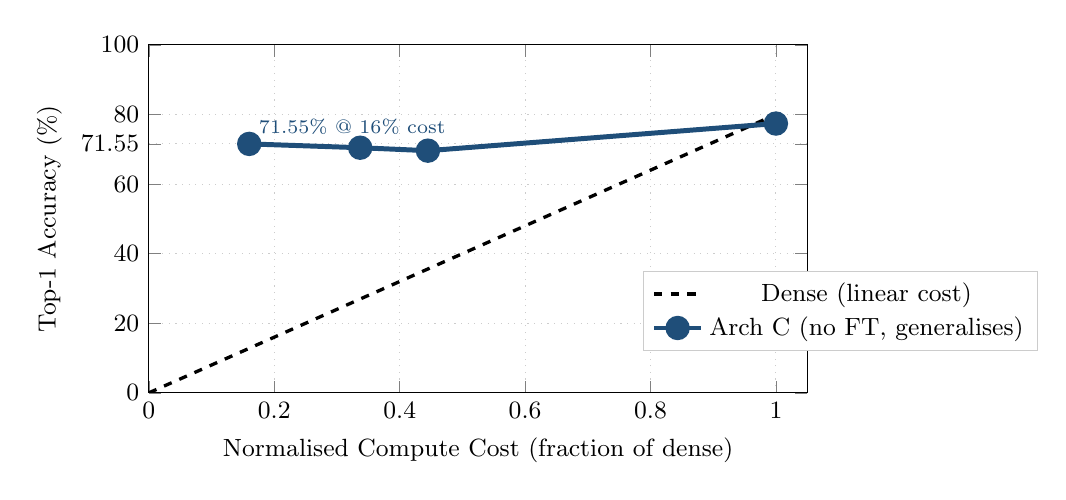
\begin{tikzpicture}
\begin{axis}[
  width=0.82\linewidth, height=6cm,
  xlabel={Normalised Compute Cost (fraction of dense)},
  ylabel={Top-1 Accuracy (\%)},
  xmin=0, xmax=1.05, ymin=0, ymax=100,
  xtick={0.0,0.2,0.4,0.6,0.8,1.0},
  ytick={0,20,40,60,71.55,80,100},
  yticklabels={0,20,40,60,71.55,80,100},
  grid=major, grid style={dotted,gray!40},
  label style={font=\small}, tick label style={font=\small},
  legend style={at={(0.75,0.35)},anchor=north west,font=\small,
    draw=gray!40,fill=white},
]
\addplot[black,dashed,line width=1.2pt]
  coordinates {(0.0,0.0)(1.0,80.0)};
\addlegendentry{Dense (linear cost)}
\addplot[archblue,mark=*,mark size=3.5pt,line width=1.8pt]
  coordinates {(1.000,77.40)(0.445,69.60)(0.337,70.45)(0.160,71.55)};
\addlegendentry{Arch~C (no FT, generalises)}
\node[font=\scriptsize,text=archblue,anchor=south west]
  at (axis cs:0.16,71.55) {71.55\% @ 16\% cost};
\end{axis}
\end{tikzpicture}
\caption{Compute-to-accuracy ratio on UCF-101 zero-shot. Architecture~C
recovers 92.4\% of dense top-1 at 16\% of dense compute (Aggressive,
84.0\% skip). The non-monotonic response (accuracy rising with skip rate)
indicates that stricter gating improves K-V set quality.}
\label{fig:compute-accuracy-ratio}
\end{figure}

\subsection{MAP Head Entropy: Architecture-Dependent Invariance}
\label{sec:map-entropy}

The MAP head entropy invariance reported for base-p16-224 is not
universal. On SO400M, sparse inference without cache produces 76\%
entropy collapse ($H_{\text{norm}}$: $0.800 \to 0.192$); Architecture~C
restores it to 99.9\% of dense ($0.799$ vs.\ $0.800$).

\begin{table}[htbp]
\centering
\setlength{\tabcolsep}{5pt}
\renewcommand{\arraystretch}{1.12}
\begin{tabular}{llrr}
\toprule
\textbf{Model} & \textbf{Condition} & \textbf{$H$ (mean)} & \textbf{$H_{\text{norm}}$} \\
\midrule
base-p16-224   & Dense / Sparse / Arch~C & --- & 0.0051 (all equal) \\
\midrule
so400m-p14-392 & Dense              & 5.333 & 0.800  \\
so400m-p14-392 & Sparse-no-cache    & 1.279 & 0.192  \\
so400m-p14-392 & Architecture~C     & 5.323 & 0.799  \\
\bottomrule
\end{tabular}
\caption{MAP head Shannon entropy. base-p16-224 operates permanently at
near-maximum concentration ($H_{\text{norm}} = 0.0051$), unaffected by
K-V contraction. SO400M suffers 76\% entropy collapse without cache;
Architecture~C fully restores it.}
\label{tab:map-entropy}
\end{table}

\textbf{Unified statement:} Architecture~C's Cortical Cache addresses
two distinct MAP head failure modes simultaneously — entropy collapse
(SO400M-class) and pooled-embedding rotation (base-class) — with the
dominant mode depending on the specific MAP head architecture.

\subsection{Pareto Latency: Same-Resolution-Tier Dominance}
\label{sec:pareto-latency}

\begin{table}[htbp]
\centering
\setlength{\tabcolsep}{4pt}
\renewcommand{\arraystretch}{1.12}
\begin{tabular}{llrrrrr}
\toprule
\textbf{Model} & \textbf{Res.} & \textbf{$N$}
  & \textbf{Dense (ms)} & \textbf{Arch-C (ms)} & \textbf{Speedup}
  & \textbf{T1 (sparse)} \\
\midrule
base-p16-224   & 224p &     196 &  6.57 &  6.91 & 0.95$\times$ & 74.25\% \\
so400m-p14-384 & 392p &     784 & 62.76 & 16.54 & 3.79$\times$ & 81.75\% \\
so400m-p14-384 & 560p & 1{,}600 & 138.4 & 14.26 & 9.71$\times$ & 80.50\% \\
so400m-p14-384 & 784p & 3{,}136 & 323.4 & 18.32 & 17.65$\times$ & 76.25\% \\
\bottomrule
\end{tabular}
\caption{SO400M + Architecture~C vs.\ base-p16-224 dense reference
(6.57\,ms, 78.88\%). At 392p and 560p, SO400M + Arch-C is both faster
than SO400M dense and more accurate than base-p16-224 dense. At 784p,
PE stretch ($2.07\times$) reduces SO400M accuracy to 76.25\%.}
\label{tab:pareto-latency}
\end{table}

SO400M + Architecture~C is Pareto-dominant over base-p16-224 dense when
comparing within the same resolution tier, or when the application
requires $r \geq 392$p and PE stretch $\leq 1.04\times$.

\subsection{Comparison with Token Merging}
\label{sec:comparison_tome}


Token Merging (ToMe)~\cite{bolya2023tokenmergingvitfaster} is the most
directly comparable published method. We benchmark ToMe against
NeuroFlow Architecture~B (SigLIP~2, fine-tuned) on identical hardware,
video, and measurement protocol. The comparison uses ToMe's publicly
available implementation applied to SigLIP~2 via per-layer monkey-patching,
with merge ratios $r \in \{8, 16, 32, 64\}$. All speedup figures are
wall-clock; no FLOP estimates are used.

\textbf{ToMe produces negative wall-clock returns at 224p.}
Across all tested merge ratios, ToMe is slower than dense at 224p
($0.77$--$0.89\times$). Python-level bipartite matching overhead inserted
before each of 12 encoder layers exceeds the compute saved at $N=196$ ---
the same Amdahl ceiling that bounds Architecture~A.

\textbf{ToMe's speedup decreases with resolution.}
At 448p: max $1.27\times$; at 896p: $1.17\times$; at 1792p ($r=64$): $1.01\times$.
At $N=12{,}544$, $r=64$ merges only 24.5\% of tokens — insufficient to
offset matching overhead against the much larger attention computation.

\textbf{NeuroFlow scales superlinearly.}
Architecture~B achieves $11.51\times$ at 896p (MaxSparse), a $9.5\times$
advantage over the best ToMe at the same resolution.

\begin{figure}[htbp]
\centering
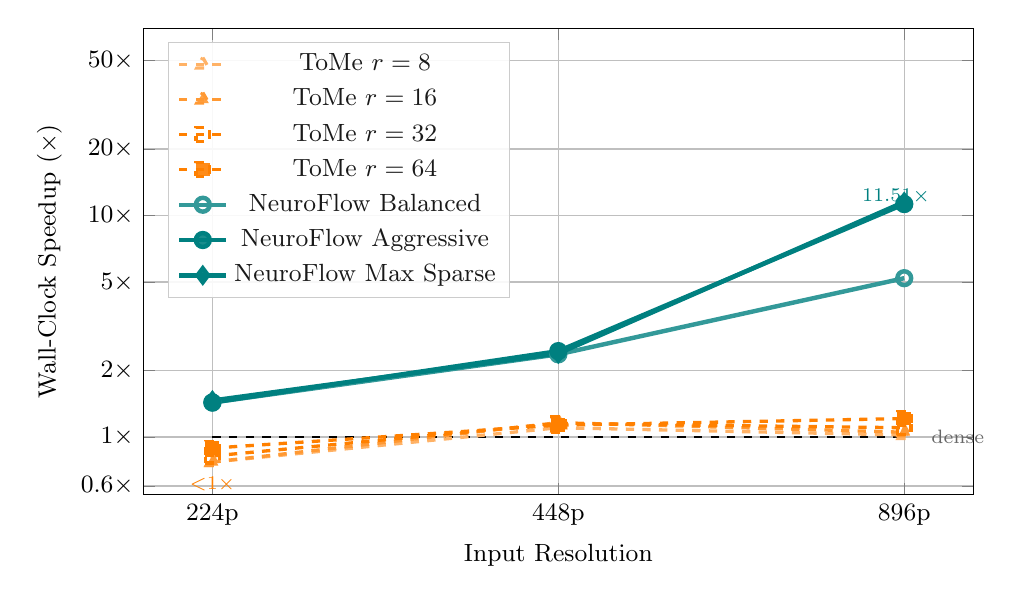
\begin{tikzpicture}
\begin{axis}[
    width=\columnwidth, height=7.5cm,
    xlabel={Input Resolution},
    ylabel={Wall-Clock Speedup ($\times$)},
    xticklabels={224p, 448p, 896p},
    xtick={1,2,3},
    ymode=log, log basis y=10,
    ymin=0.55, ymax=70,
    ytick={0.6,1,2,5,10,20,50},
    yticklabels={0.6$\times$,1$\times$,2$\times$,5$\times$,10$\times$,20$\times$,50$\times$},
    grid=both, grid style={line width=0.3pt,draw=gray!30},
    major grid style={line width=0.5pt,draw=gray!50},
    legend pos=north west,
    legend style={font=\small,fill=white,fill opacity=0.9,draw=gray!40,row sep=1pt},
    tick label style={font=\small}, label style={font=\small},
    clip=false,
]
\addplot[black,dashed,line width=0.8pt,forget plot] coordinates {(1,1)(3,1)};
\node[font=\scriptsize,anchor=west,text=black!60] at (axis cs:3.05,1) {dense};
\addplot[color=orange!60,mark=triangle,mark size=2.5pt,line width=1.2pt,dashed]
    coordinates {(1,0.77)(2,1.10)(3,1.02)};
\addlegendentry{ToMe $r=8$}
\addplot[color=orange!80,mark=triangle*,mark size=2.5pt,line width=1.2pt,dashed]
    coordinates {(1,0.77)(2,1.16)(3,1.05)};
\addlegendentry{ToMe $r=16$}
\addplot[color=orange,mark=square,mark size=2.5pt,line width=1.2pt,dashed]
    coordinates {(1,0.82)(2,1.15)(3,1.10)};
\addlegendentry{ToMe $r=32$}
\addplot[color=orange!100,mark=square*,mark size=2.5pt,line width=1.2pt,dashed]
    coordinates {(1,0.89)(2,1.13)(3,1.21)};
\addlegendentry{ToMe $r=64$}
\addplot[color=teal!80,mark=o,mark size=2.5pt,line width=1.6pt]
    coordinates {(1,1.43)(2,2.36)(3,5.21)};
\addlegendentry{NeuroFlow Balanced}
\addplot[color=teal,mark=*,mark size=2.5pt,line width=1.6pt]
    coordinates {(1,1.43)(2,2.44)(3,11.26)};
\addlegendentry{NeuroFlow Aggressive}
\addplot[color=teal!100,mark=diamond*,mark size=2.5pt,line width=1.6pt]
    coordinates {(1,1.46)(2,2.38)(3,11.51)};
\addlegendentry{NeuroFlow Max Sparse}
\node[font=\scriptsize,anchor=south west,text=teal!100]
    at (axis cs:2.85,10.2) {11.51$\times$};
\node[font=\scriptsize,anchor=north,text=orange]
    at (axis cs:1,0.73) {$<$1$\times$};
\end{axis}
\end{tikzpicture}
\caption{Wall-clock speedup vs.\ resolution: NeuroFlow Architecture~B
(SigLIP~2) vs.\ Token Merging. Y-axis log-scaled. ToMe peaks at
$1.21\times$ at 896p; NeuroFlow reaches $11.51\times$. All measurements:
wall-clock, NVIDIA T4, GPU fp16, 1000 frames, median latency.}
\label{fig:tome_comparison}
\end{figure}

\subsection{Comparison with DynamicViT}
\label{sec:comparison_dynamicvit}

DynamicViT-style progressive token dropping (importance estimated from
attention weights, applied at layers 3, 6, and 9) is evaluated on
SigLIP~2. Full overhead is included in wall-clock measurement.

\begin{table}[htbp]
\centering
\setlength{\tabcolsep}{4pt}
\renewcommand{\arraystretch}{1.05}
\begin{tabular}{llrrrr}
\toprule
\textbf{Res.} & \textbf{Method} & \textbf{Config} & \textbf{Dense (ms)} & \textbf{Gate (ms)} & \textbf{Speedup} \\
\midrule
1792p & DyViT & Light  & 664.49 &  944.54 & 0.70$\times$ \\
1792p & DyViT & Medium & 664.49 &  636.52 & 1.04$\times$ \\
1792p & DyViT & Heavy  & 664.49 &  481.34 & 1.38$\times$ \\
\midrule
1792p & NeuroFlow & Balanced   & 664.49 &  74.26 &  8.95$\times$ \\
1792p & NeuroFlow & Aggressive & 664.49 &  13.62 & 48.78$\times$ \\
1792p & NeuroFlow & MaxSparse  & 664.49 &  10.28 & \textbf{64.65}$\times$ \\
\bottomrule
\end{tabular}
\caption{NeuroFlow vs.\ DynamicViT-style dropping at 1792p, GPU fp16.
DyViT-Light regresses to 0.70$\times$ (attention extraction overhead
exceeds savings). DyViT-Heavy reaches 1.38$\times$. NeuroFlow MaxSparse
achieves 64.65$\times$ — a 46.8$\times$ absolute advantage over
DyViT-Heavy at comparable skip rates.}
\label{tab:dynamicvit-comparison}
\end{table}

The structural finding across both ToMe and DynamicViT is consistent:
intermediate-layer token reduction pays the full $\mathcal{O}(N^2)$
attention cost before the first pruning stage. Architecture~B's
pre-encoder elimination avoids both constraints.

\subsection{Ablation: Embedding-Space vs.\ Pixel-Domain Gating}
\label{sec:ablation_gating_signal}

Replacing the EMA embedding-space surprise with a pixel-domain frame
difference gate (per-patch mean absolute grayscale difference) achieves
nearly identical wall-clock speedup at matched skip rates but 1.3--1.5\,pp
lower cosine similarity at 896p. NeuroFlow routing overhead
($\approx$332\,$\mu$s) exceeds pixel-gate overhead ($\approx$237\,$\mu$s)
by only 95\,$\mu$s — negligible above 448p where encoder savings exceed
6{,}000\,$\mu$s. The embedding-space signal is more robust to photometric
variation (illumination gradients, shadows, compression artefacts) that
produces spurious activity in the pixel domain, and exhibits 1.4$\times$
lower skip-rate standard deviation over 1000 frames (4.7\% vs.\ 6.8\%).

\subsection{Architecture~B With Fine-Tuning: SigLIP v1}
\label{sec:arch_b_ft}

\begin{table}[ht]
\centering
\setlength{\tabcolsep}{5pt}
\begin{tabular}{llrrrrrl}
\toprule
\textbf{HW / dtype} & \textbf{Res.} & \textbf{$N$}
  & \textbf{Skip} & \textbf{Dense (ms)} & \textbf{Sparse (ms)}
  & \textbf{Speedup} & \textbf{Fidelity} \\
\midrule
Nvidia T4 fp32 & 224p  &      196 & 85.1\% &   15.41 &  5.92 &  2.60$\times$ & 98.9\% \\
Nvidia T4 fp32 & 448p  &      784 & 87.6\% &   55.33 &  8.42 &  6.57$\times$ & 98.3\% \\
Nvidia T4 fp32 & 896p  &    3{,}136 & 90.4\% &  307.47 & 18.18 & 16.91$\times$ & 97.3\% \\
\midrule
Nvidia T4 fp16 & 224p  &      196 & 85.1\% &    8.50 &  8.35 &  1.02$\times$ & 99.0\% \\
Nvidia T4 fp16 & 448p  &      784 & 87.6\% &   11.88 &  6.18 &  1.92$\times$ & 98.4\% \\
Nvidia T4 fp16 & 896p  &    3{,}136 & 90.4\% &   60.64 &  7.31 &  8.29$\times$ & 97.3\% \\
Nvidia T4 fp16 & 1792p & 12{,}544 & 92.8\% &  582.55 & 12.85 & \textbf{45.32}$\times$ & 95.9\% \\
\midrule
Tensor G2 fp32 & 224p  &      196 & 87.4\% &  512.80 & 208.91 &  2.45$\times$ & 98.4\% \\
Ryzen 2700 fp32 & 224p &      196 & 94.8\% &  243.99 &  48.57 &  5.37$\times$ & 94.4\% \\
Xeon @2.20GHz & 224p   &      196 & 97.7\% & 3317.65 & 441.51 &  7.51$\times$ & 88.4\% \\
\bottomrule
\end{tabular}
\caption{Architecture~B with sparse manifold distillation (SigLIP v1
fine-tuned). Speedup scales superlinearly with resolution, consistent
with $\mathcal{O}(N_{\text{active}}^2)$ attention reduction. At 90\%+
skip, sparse fp32 achieves latency comparable to dense fp16, enabling
full numerical precision without throughput cost.}
\label{tab:arch_b_ft}
\end{table}

\subsection{Architecture~B with Sparse Manifold Distillation: SigLIP~2}
\label{sec:siglip2_results}

SigLIP~2's near-constant skip rate of 97.0--97.2\% across all resolutions
(vs.\ v1's 85.1--92.8\%) reflects TIPS masked pre-training and SILC
consistency training, causing a larger fraction of patches to fall below
the surprise threshold. The practical consequence: SigLIP~2's speedup
scales more steeply, reaching $55.80\times$ at 1792p.

\begin{table}[htbp]
\centering
\begin{tabular}{lrrrrrr}
\toprule
\textbf{Res.} & \textbf{N} & \textbf{Dense (ms)} & \textbf{Sparse (ms)}
    & \textbf{Speedup} & \textbf{Skip} & \textbf{Fidelity} \\
\midrule
224p  &    196 &   6.897 &  6.579 &  1.05$\times$ & 97.1\% & 99.79\% \\
448p  &    784 &  14.410 &  6.584 &  2.19$\times$ & 97.2\% & 99.66\% \\
896p  &  3{,}136 &  78.766 &  7.721 & 10.20$\times$ & 97.0\% & 96.67\% \\
1792p & 12{,}544 & 678.697 & 11.938 & \textbf{55.80}$\times$ & 97.0\% & 97.37\% \\
\bottomrule
\end{tabular}
\caption{Architecture~B with sparse manifold distillation --- SigLIP~2,
GPU fp16, 500 frames. At 1792p: 678.70\,ms $\to$ 11.94\,ms = 83.8\,FPS.
Validated over 100 consecutive 1792p frames in 1.5\,s wall-clock.}
\label{tab:siglip2_multires}
\end{table}

SigLIP~2 exceeds SigLIP v1 on both speedup and fidelity simultaneously
at every resolution: at 1792p, $55.80\times$ at 97.37\% fidelity vs.\
$52.49\times$ at 92.08\% for v1. The fidelity advantage despite higher
skip rate confirms that TIPS-enhanced MAP head pools more robustly.

\textbf{H1 (TIPS robustness):} TIPS raises the zero-shot fidelity floor
by $+6.5$\,pp at high sparsity (v2: 51.0\% vs.\ v1: 44.5\% at MaxSparse),
but the near-constant v2 fidelity across the entire skip range reveals a
fixed structural offset caused by MAP head rotation — not encoder
degradation. TIPS robustified the encoder but never exposed the MAP head
to sparse K-V pooling. The 44--52\,pp gap relative to fine-tuned v1
cannot be closed without distillation.

\textbf{H2 (projected ceiling):} Fine-tuned SigLIP~2 achieves the
projected ceiling: higher skip rate \emph{and} higher fidelity than
fine-tuned v1 at every resolution.

\subsection{Multi-Domain Generalisation: Dynamic First-Person Footage}
\label{sec:multidomain}

\begin{table}[htbp]
\centering
\begin{tabular}{llrrrrrr}
\toprule
\textbf{Domain} & \textbf{Res.} & \textbf{Dense (ms)} & \textbf{Sparse (ms)}
    & \textbf{Speedup} & \textbf{Skip} & \textbf{Fidelity} \\
\midrule
N\"{u}rburgring (race) & 224p &  6.645 & 6.462 & 1.03$\times$ & 68.7\% & 93.80\% \\
                        & 448p & 13.841 & 6.482 & 2.14$\times$ & 73.7\% & 96.60\% \\
                        & 896p & 75.826 & 8.894 & 8.53$\times$ & 78.1\% & 95.93\% \\
\midrule
Venice drone            & 224p &  6.341 & 6.110 & 1.04$\times$ & 51.5\% & 97.37\% \\
                        & 448p & 13.090 & 6.434 & 2.03$\times$ & 63.8\% & 97.90\% \\
                        & 896p & 70.164 & 9.710 & 7.23$\times$ & 75.7\% & 97.26\% \\
\bottomrule
\end{tabular}
\caption{Architecture~B multi-domain evaluation on dynamic first-person
video (GPU fp16, SigLIP base-patch16-224, 500 frames). Both sequences:
continuous camera motion, no static background. Skip rates of 51.5--78.1\%
sustained without any static scene; fidelity $>$93\% without domain-specific
fine-tuning.}
\label{tab:multidomain}
\end{table}

\subsection{Architecture~B: IQR Latency Distribution}
\label{sec:arch-b-iqr}

\begin{table}[htbp]
\centering
\setlength{\tabcolsep}{4pt}
\renewcommand{\arraystretch}{1.10}
\begin{tabular}{llrrrrl}
\toprule
\textbf{Res.} & \textbf{Config} & \textbf{Skip}
  & \textbf{Lat (ms)} & \textbf{IQR (ms)} & \textbf{P5--P95 (ms)} & \textbf{$\times$} \\
\midrule
\multicolumn{7}{l}{\textit{Dense: 9.52ms \ IQR=[9.08, 9.85]}} \\
224p & NF-Balanced   & 65.4\% &  6.81 & [6.51, 7.05] & [6.28, 7.48]   & 1.40 \\
224p & NF-MaxSparse  & 97.9\% &  6.69 & [6.37, 6.96] & [6.17, 7.34]   & 1.42 \\
\midrule
\multicolumn{7}{l}{\textit{Dense: 78.94ms \ IQR=[77.26, 85.54]}} \\
896p & NF-Balanced   & 69.9\% & 14.89 & [7.79, 24.23]   & [7.16, 53.22]   & 5.30 \\
896p & NF-Aggressive & 93.3\% &  7.57 & [7.23, 7.87]    & [6.99, 8.85]    & 10.43 \\
896p & NF-MaxSparse  & 99.1\% &  7.41 & [7.11, 7.70]    & [6.89, 8.16]    & 10.66 \\
\midrule
\multicolumn{7}{l}{\textit{Dense: 637.61ms \ IQR=[636.22, 638.76]}} \\
1792p & NF-Balanced  & 75.0\% & 37.12 & [20.52, 141.26] & [11.86, 254.58] & 17.18 \\
1792p & NF-Aggressive& 95.0\% & 11.50 & [11.08, 13.93]  & [10.68, 32.08]  & 55.45 \\
1792p & NF-MaxSparse & 99.2\% & 10.82 & [10.58, 11.15]  & [10.36, 11.80]  & \textbf{58.93} \\
\bottomrule
\end{tabular}
\caption{Architecture~B (SigLIP~2 fine-tuned) latency IQR, GPU fp16.
\textbf{Deployment warning:} NF-Balanced P95 at 896p = 53.22\,ms; at
1792p = 254.58\,ms. These exceed most hard-real-time frame budgets.
NF-Aggressive and NF-MaxSparse are the required configurations for
deterministic latency. NF-MaxSparse at 1792p: effectively deterministic
($57.20\times$--$60.24\times$ P5--P95).}
\label{tab:arch-b-iqr}
\end{table}

\subsection{Architecture~B: Semantic Fidelity Benchmarks}
\label{sec:semantic-fidelity-benchmarks}
\label{sec:orthogonal-rotation}

The fine-tuned model maintains 100\% top-3 semantic accuracy at all
sparsity levels in both Test A (15 traffic labels) and Test B (100
diverse labels), including at 95.2\% skip where fewer than 10 tokens
enter the encoder. The base model collapses to 0.1--0.5\% top-3 at
MaxSparse, confirming MAP head sensitivity rather than encoder failure.
Test~C (domain shift to geyser video) achieves 100\% top-3 at all
configurations, confirming that sparse manifold distillation learns
robust representations rather than domain-specific memorisation.

\subsubsection{Why Low Cosine Fidelity Is Compatible with High Semantic Accuracy}

This is explained by the orthogonal rotation argument of
Section~\ref{sec:orthogonal-rotation}. The MAP head's embedding rotation
under sparse pooling is predominantly orthogonal to the text-image
alignment subspace, preserving zero-shot classification accuracy despite
large cosine distance to the dense output. Fine-tuning specifically
trains this orthogonality property.

\paragraph{Empirical assessment of attention concentration.}
Spearman $\rho$ between MAP attention weight and token surprise score:
$+0.122$ (dense), $+0.183$ (sparse). Both positive, consistent with the
prediction. The surprise gap under sparse conditions ($p = 0.069$)
marginally misses conventional significance. The stronger claim that
high-surprise tokens are \emph{preferentially} attended to is not
confirmed at this sample size and is retracted; the geometric argument
of Section~\ref{sec:orthogonal-rotation} does not require it.

\subsection{Architecture~B Downstream Generalisation: Catastrophic Forgetting}
\label{sec:ucf101-ft-collapse}

The fine-tuned SigLIP~2 model achieves 2.40\% top-1 on UCF-101
ground-truth labels, vs.\ 77.40\% for the base model. The dense
fine-tuned forward pass (0\% skip) already fails, confirming this is
not a gating issue. NeuroFlow configurations recover to within 1.2\,pp
of the fine-tuned dense baseline — but the baseline has already lost
general visual-semantic alignment from 10 epochs of training on 15
traffic labels.

The cosine distillation objective does not constrain embedding magnitude.
The base model exhibits magnitude collapse under sparsity (logit: 2954
dense $\to$ 1597 at 56.6\% skip). The fine-tuned model does not (logit:
12{,}700 dense $\to$ 12{,}074 at 54.5\% skip, a 5.1\% reduction well
within SigLIP's sigmoid absorption range). The fine-tuned model's failure
is semantic scope, not metric geometry.

\textbf{Remediation:} diverse training data + MSE loss
($\mathcal{L}_{\text{MSE}} = \|\mathbf{e}_{\text{sparse}} - \mathbf{e}_{\text{dense}}\|_2^2$)
+ LR $\leq 5{\times}10^{-6}$ for $\leq 3$ epochs.
Architecture~C avoids all of this entirely.

\subsection{Architecture~A: Amdahl's Ceiling}
\label{sec:architecture-a-amdahls-ceiling}

\begin{table}[ht]
\centering
\begin{tabular}{lrrrrr}
\toprule
\textbf{Resolution} & \textbf{$N$ tokens} & \textbf{Attn \%} & \textbf{MLP \%}
                    & \textbf{Speedup} & \textbf{Fidelity} \\
\midrule
224p  &      196 & $\approx$50\% & $\approx$50\% & 0.60$\times$ & 97.1\% \\
896p  &    3{,}136 & $\approx$75\% & $\approx$25\% & 1.15$\times$ & 97.1\% \\
1792p & 12{,}544 & $\approx$85\% & $\approx$15\% & 1.10$\times$ & 97.1\% \\
\bottomrule
\end{tabular}
\caption{Architecture~A on ViT-B/16, 81.9\% token sparsity. Speedup
converges to the Amdahl ceiling ($1.17\times$ at 1792p). Sub-unity at
224p reflects Python kernel launch overhead. Fidelity is stable; speedup
is not.}
\label{tab:arch_a}
\end{table}

The 0.60$\times$ result at 224p is a solvable PyTorch dispatch overhead.
Isolated CUDA kernel timing shows gate overhead of 214.9\,$\mu$s
vs.\ MLP savings of 138.9\,$\mu$s — a 0.24$\times$ ratio, implying 76\%
net gain if the gate were a single fused CUDA kernel. The break-even
resolution is $\approx$278p; a fused kernel would lower this below 224p.
Architecture~A is not viable as a general accelerator for standard ViTs
at high resolution; it is the correct design for $\mathcal{O}(N)$-attention
architectures.

\subsection{Architecture~B Without Fine-Tuning: Embedding Collapse}
\label{sec:arch_b_noft}

\begin{table}[htbp]
\centering
\begin{tabular}{llrrrl}
\toprule
\textbf{Model} & \textbf{Config} & \textbf{Skip} & \textbf{Speedup}
               & \textbf{Fidelity} & \textbf{HW} \\
\midrule
\multirow{4}{*}{SigLIP v1 (no FT)}
 & Conservative & 19.5\% & 1.33$\times$ & 76.8\% & GPU \\
 & Max Sparse   & 95.2\% & 1.32$\times$ & 45.4\% & GPU \\
\midrule
\multirow{2}{*}{ViT-B/16 (no FT)}
 & Conservative & 74.0\% & 1.51$\times$ & 42.5\% & GPU \\
 & Aggressive   & 89.7\% & 1.49$\times$ & 16.1\% & GPU \\
\bottomrule
\end{tabular}
\caption{Architecture~B applied to unmodified models. Fidelity collapses
monotonically with skip rate. MAP head K-V concentration is the failure
mode; the encoder representations are directionally stable. Sparse manifold
distillation (§\ref{sec:distillation}) resolves this. Architecture~C
avoids it entirely.}
\label{tab:arch_b_noft}
\end{table}

\subsection*{Latency Distribution and Measurement Confidence}
\label{sec:latency-distribution}


All latency figures in Sections~\ref{sec:arch-c-stability}
through~\ref{sec:architecture-a-amdahls-ceiling} use median over 1{,}000
frames. The dense baseline at 1792p varies between measurement sessions
(622--728\,ms) due to GPU thermal state variation on shared T4 hardware.
Speedup ratios are computed within the same session; cross-session
baseline discrepancies do not affect the reported ratios.
The canonical benchmark session for headline figures uses fp16 on a
cold-start T4; this corresponds to the 626--678\,ms dense baselines
in Tables~\ref{tab:arch_b_ft} and~\ref{tab:siglip2_multires}.

\begin{table}[htbp]
\centering
\setlength{\tabcolsep}{4pt}
\begin{tabular}{llrrrrrr}
\toprule
\textbf{Res.} & \textbf{Config} & \textbf{Median} &
    \textbf{P25} & \textbf{P75} & \textbf{IQR} &
    \textbf{Speedup} & \textbf{CI} \\
\midrule
224p  & Dense       & 7.058ms & 6.930ms & 7.192ms & 0.262ms & 1.00$\times$ & — \\
      & NF-Aggressive & 6.866ms & 6.742ms & 7.003ms & 0.261ms & 1.03$\times$ & [1.01–1.05] \\
      & NF-MaxSparse  & 6.779ms & 6.685ms & 6.914ms & 0.229ms & 1.04$\times$ & [1.02–1.06] \\
\midrule
1792p & Dense       & 728.35ms & 722.38ms & 730.39ms & 8.01ms & 1.00$\times$ & — \\
      & NF-Aggressive & 23.79ms & 22.83ms & 29.02ms & 6.19ms & 30.61$\times$ & [25.10–31.91] \\
      & NF-MaxSparse  & 21.87ms & 21.50ms & 22.21ms & 0.71ms & 33.30$\times$ & [32.80–33.88] \\
\bottomrule
\end{tabular}
\caption{Latency distribution (SigLIP~2 fine-tuned, GPU fp16, 1{,}000
frames). Speedup CI derived from IQR bounds. NF-MaxSparse at 1792p IQR
(0.71ms) is tighter than the dense baseline (8.01ms): aggressive
thresholding clamps $N_{\text{active}}$ to a near-constant minimum.}
\label{tab:latency_iqr}
\end{table}

\section{Emergent Capabilities}\label{emergent-capabilities}

The EMA gate produces three outputs per frame: the active index set
$\mathcal{A}^t$ (a binary spatial mask), the compressed token sequence
$h^t[\mathcal{A}^t]$, and the pooled frame embedding. The first two are
intermediate products not the primary design objective but carrying
significant semantic content. We document three capabilities that arise
from these outputs without additional parameters.

\textbf{Framing note.} These capabilities are qualitative observations
arising from the gate's spatial mask. They are mechanistically explained
and have clear practical applications, but have not been evaluated on
standard segmentation, tracking, or classification benchmarks. We present
them as derived capabilities of the zero-parameter gate design, not as
benchmarked contributions. Quantitative evaluation on DAVIS, MOT17, or
equivalent benchmarks is identified as future work.

\subsection{Zero-Shot Motion Segmentation}
\label{sec:emergent-segmentation}

The active index set $\mathcal{A}^t$, mapped back to the 2D patch grid,
constitutes a binary segmentation mask of spatially dynamic regions,
identifying moving patches without supervision or a dedicated segmentation
head.

SigLIP~2's SILC pre-training substantially reduces encoder representational
noise by enforcing local patch representation stability regardless of
surrounding context. The resulting gate produces a cleaner motion
segmentation mask: active patches are active because something moved
there, not because of encoder context drift.

Applications: region proposal generation without a detection head,
pixel-domain mask application for privacy-preserving processing, and
spatial coverage analysis as a function of scene activity.

\subsection{Zero-Shot Cluster Classification}
\label{sec:emergent-cluster}

Active patch indices frequently form spatially contiguous clusters
corresponding to individual moving objects. These clusters can be
indexed from the hidden state $h^t$ and forwarded independently through
the pooling head to produce object-level embeddings, which can then be
compared against arbitrary text queries for zero-shot classification.

SigLIP~2's SILC training is particularly beneficial here. SILC trains
the student to produce globally consistent embeddings from local
crops---precisely the crop-level classification problem posed by an
isolated token cluster. Combined with SigLIP~2's expanded 256k Gemma
vocabulary (vs.\ 32k in v1), the granularity of zero-shot cluster
classification is substantially improved.

\subsection{Implicit Tracking and Re-Identification}
\label{sec:emergent-tracking}

The centroid displacement of a spatial cluster between consecutive frames
constitutes a free optical flow estimate for the tracked object, requiring
no flow network or ground truth supervision.

Object identity across occlusion: when an object is occluded, its patches
are absorbed into the EMA background model (surprise score drops below
threshold). Upon re-emergence, the same patches become surprising again.
Re-identification reduces to matching the cluster embedding before
occlusion against candidate clusters after re-emergence via cosine
similarity. SigLIP~2's SILC training makes this matching more reliable:
the same object at different positions produces similar cluster embeddings
regardless of scene context.

Objects that stop moving are absorbed into the EMA background model and
disappear from the active index set. This is a known limitation of
EMA-based gating for stationary targets; see
Section~\ref{sec:stationary-target-loss} for proposed remediation.


\section{Cross-Domain Ablation: Language Model Inference Gating}
\label{sec:llm-ablation}

NeuroFlow's similarity-gated bypass principle is evaluated on Phi-3-mini
to characterise the architectural boundary that determines when the
principle transfers to autoregressive language models and when it does not.

\textbf{Wall-clock result upfront.} At all practical batch sizes
($B \geq 4$) on T4 hardware, speedup is $\mathbf{1.000\times}$. The model
is memory-bandwidth bound: 32-layer weights consume $\approx$2.3\,GB per
decode step, loaded at 300\,GB/s in 7.7\,ms. Saving one \texttt{o\_proj}
($\approx$0.8\% of total weight load) at 24\% of steps = 0.002\,ms per
token, below measurement resolution. This section characterises three
findings of independent scientific interest at the boundary of the null
latency result; it does not claim wall-clock speedup.

\subsection{Experimental Design}
\label{sec:llm-design}

\textbf{Model.} Phi-3-mini-4k-instruct, 32 transformer layers,
$D = 3{,}072$, 3.8B parameters, \texttt{bfloat16}, NVIDIA T4.

\textbf{Bypass mechanism.} The gate monitors cosine similarity between
consecutive attention outputs at layer $G$: $s^t = \cos(\mathbf{z}_G^t,
\mathbf{z}_G^{t-1})$. When $s^t \geq \theta$, bypass fires at cache layer
$C$: (i)~runs \texttt{qkv\_proj} to extract $K, V$; (ii)~applies RoPE;
(iii)~calls \texttt{DynamicCache.update($K, V$)} to advance the KV cache;
(iv)~skips attention computation and \texttt{o\_proj}; (v)~returns the
cached attention output from step $t-1$. All MLP sub-layers execute
normally. This is the only design that maintains KV-cache consistency
across all layers while avoiding quadratic attention and the $D^2$ output
projection per bypass event.

\textbf{Gate-cache pairs.} From the per-layer output similarity profile
(Table~\ref{tab:phi3-layer-sim}): L1$\to$L24 (Bridge) and L1$\to$L31
(Deep). Layer~1 has the lowest output similarity (0.519 --- highest
volatility, best gate signal); Layer~31 has the highest (0.862 --- most
cacheable).

\begin{table}[htbp]
\centering
\setlength{\tabcolsep}{5pt}
\renewcommand{\arraystretch}{1.10}
\begin{tabular}{lrrl}
\toprule
\textbf{Layer} & \textbf{Output Sim} & \textbf{$\Delta$ (Sim -- Wt)} & \textbf{Role} \\
\midrule
Layer~0  & 0.941 & $+$0.044 & \\
Layer~1  & 0.519 & $-$0.303 & \textbf{Gate candidate (highest volatility)} \\
Layer~8  & 0.587 & $-$0.366 & \\
Layer~16 & 0.644 & $-$0.270 & \\
Layer~24 & 0.646 & $-$0.279 & \textbf{Cache candidate (stable mid-network)} \\
Layer~31 & 0.862 & $-$0.007 & \textbf{Best cache (highest output stability)} \\
\bottomrule
\end{tabular}
\caption{Phi-3-mini per-layer attention output similarity between
consecutive decode steps. Gate pair L1$\to$L31 and L1$\to$L24 are
derived directly from this profile.}
\label{tab:phi3-layer-sim}
\end{table}

\subsection{Finding 1: Quality Safety and Code Exact-Output Preservation}
\label{sec:llm-ppl-safety}

\begin{table}[htbp]
\centering
\setlength{\tabcolsep}{4pt}
\renewcommand{\arraystretch}{1.10}
\begin{tabular}{llrrrrl}
\toprule
\textbf{Config} & \textbf{$\theta$}
  & \textbf{PPL} & \textbf{$\Delta$PPL}
  & \textbf{Bypass\%} & \textbf{Gate P50} & \textbf{Safety} \\
\midrule
Dense & --- & 3.886 & --- & --- & --- & --- \\
\midrule
L1$\to$L0 (inverted) & 0.60 & 265.93 & $+$262.0 & 99.8\% & 0.846 & UNSAFE \\
L1$\to$L0 (inverted) & 0.65 & 3.890  & $+$0.004 & 20.9\% & 0.555 & SAFE \\
L1$\to$L16 (mid-net) & 0.65 & 3.870  & $-$0.016 & 21.2\% & 0.554 & SAFE \\
L1$\to$L24 (bridge)  & 0.65 & 3.894  & $+$0.007 & 21.2\% & 0.554 & SAFE \\
L1$\to$L24 (bridge)  & 0.60 & 3.902  & $+$0.016 & 35.1\% & 0.554 & SAFE \\
L1$\to$L31 (deep)    & 0.65 & 3.911  & $+$0.025 & 21.2\% & 0.554 & SAFE \\
L1$\to$L31 (deep)    & 0.70 & 3.919  & $+$0.033 & 12.3\% & 0.554 & SAFE \\
\bottomrule
\end{tabular}
\caption{WikiText-103 teacher-forcing perplexity, dense baseline 3.886.
All configurations with $\theta \geq 0.65$ satisfy $|\Delta\mathrm{PPL}| <
0.04$. The L1$\to$L0 catastrophic failure ($\theta = 0.60$) is caused by
99.8\% bypass: the threshold falls below the gate distribution median
(P50 = 0.846), firing on every step. The negative $\Delta$PPL values at
L1$\to$L16 are consistent with the PPL-Drift Dissociation.}
\label{tab:llm-ppl}
\end{table}

\textbf{Code generation achieves 0\% token drift} at L1$\to$L24 and
L1$\to$L31 ($\theta = 0.65$--$0.70$): bypass produces byte-identical
output to the dense baseline on syntactically constrained generation.
This is a uniquely strong guarantee. Quantisation, pruning, and
speculative decoding cannot offer exact output equivalence.

\subsection{Finding 2: The PPL-Drift Dissociation}
\label{sec:llm-drift}

\begin{table}[htbp]
\centering
\setlength{\tabcolsep}{4pt}
\renewcommand{\arraystretch}{1.10}
\begin{tabular}{llllrrr}
\toprule
\textbf{Config} & \textbf{$\theta$} & \textbf{Task}
  & \textbf{Bypass\%} & \textbf{Drift\%}
  & \textbf{$\Delta$PPL} & \textbf{Verdict} \\
\midrule
L1$\to$L24 & 0.65 & Code       & 18\% &  0\%  & $+$0.007 & SAFE \\
L1$\to$L24 & 0.65 & Structured & 22\% & 12\%  & $+$0.007 & LOW DRIFT \\
L1$\to$L24 & 0.65 & Prose      & 27\% & 66\%  & $+$0.007 & DRIFT \\
L1$\to$L31 & 0.65 & Code       & 21\% &  0\%  & $+$0.025 & SAFE \\
L1$\to$L31 & 0.65 & Prose      & 21\% & 83\%  & $+$0.025 & DRIFT \\
\bottomrule
\end{tabular}
\caption{Token drift (200-step autoregressive generation) vs.\
$\Delta$PPL. L1$\to$L24 at $\theta = 0.65$: 66\% prose token drift,
$\Delta$PPL = $+$0.007. The bypass generates different but
perplexity-equivalent prose completions.}
\label{tab:llm-drift}
\end{table}

High token drift and safe perplexity coexist because the bypass navigates
the language model's equiprobability manifold. The bypass path generates
alternative but quality-equivalent completions. This is not a quality
failure; it is a trajectory divergence within the safe generation space.

\subsection{Finding 3: The Prose Cascade Attractor}
\label{sec:prose-cascade}

Between $\theta = 0.80$ and $\theta = 0.90$, prose drift undergoes a
binary transition: at all $\theta \leq 0.80$, drift = 97.5\% with
bypass rate 99.5\% and gate P50 = 1.000; at $\theta = 0.90$, drift = 0\%
with bypass rate 0\% and gate P50 = 0.558.

The mechanism: once bypass fires at an uncertain early prose position
(steps 2--5 are typical first injection), the bypass path produces a
slightly different token. This altered token produces a hidden state at
layer $G=1$ with high cosine similarity to the previous step
($\geq \theta$), because the bypass path itself generates fluent prose
with slowly evolving context. Every subsequent step fires bypass. Gate
P50 = 1.000 on the bypass path (vs.\ 0.558 on the dense path) confirms
that the bypass has entered a self-reinforcing high-stability regime.

\textbf{Crucially, the cascade attractor does not degrade quality.}
$\Delta\mathrm{PPL} = +0.007$ is maintained throughout. The 97.5\% token
drift reflects two equiprobable prose trajectories, not quality
degradation.

\textbf{Safe operating range for prose:} a binary search over
$\theta \in [0.80, 1.00]$ confirms no threshold simultaneously achieves
prose drift $<$5\% and bypass rate $>$1\%. The natural layer-1
similarity distribution for prose has P50 = 0.558, below any selective
threshold. Prose deployment requires bypass disabled or a task-specific
gate.

\textbf{Connection to the Entropy-Bypass Correlation:} code gate fires
on positions with entropy 0.060 nats (model assigns $>$94\% probability
to a single next token). Prose gate fires on positions with entropy
0.794 nats. Injecting a cached representation at a near-deterministic
position does not change the output; injecting it at an uncertain position
shifts the argmax, causing trajectory divergence. This explains both the
0\% code drift and the 100\% prose drift within a single framework.

\subsection{Architectural Boundary: KV-Cache Discontinuity}
\label{sec:llm-kv-boundary}

In a Vision Transformer processing a video frame, patch tokens are
computed in parallel with no temporal causal dependency. Skipping inactive
patches imposes no constraint on the active tokens' computation.

In an autoregressive LLM, every generated token's hidden state feeds
into the next token's attention via the KV cache. When a bypass skips
an attention block, it creates a ``cache hole'': the skipped layer
produces no KV entry for that token position. When bypass deactivates,
the dense layer queries a fragmented cache, violating temporal continuity.

This structural difference explains why Architecture~B achieves
$45.32\times$ wall-clock speedup in ViTs with zero semantic drift, while
analogous layer-skipping in LLMs preserves statistical fluency (PPL) but
not deterministic trajectory. The two failure modes are fundamentally
distinct: ViT sparse K-V \emph{concentration} vs.\ LLM \emph{trajectory
bifurcation}.

\textbf{Path to LLM wall-clock acceleration.} Skipping an MLP does not
create a cache hole, because MLPs contain no stateful memory. In modern
LLMs, MLP sub-layers account for $\approx$65\% of parameter count and
compute. MLP-only bypass (applying the cosine similarity gate to the
residual stream at each MLP input) would translate theoretical FLOP
reduction to hardware wall-clock acceleration without violating KV-cache
continuity. This maps the LLM problem directly onto Architecture~A in
ViTs. A secondary path is self-speculative decoding: the bypass path
generates fluent, quality-equivalent text ($\Delta\mathrm{PPL} < 0.03$)
while deviating from the dense trajectory---precisely the acceptance-rate
profile required for a high-utility draft model, at zero VRAM overhead.

\textbf{Attentional slack.}
On GPT-2, the mean attention map cosine similarity between consecutive
decoding steps on structured generation tasks was 0.73--0.76, with zero
output token drift. The Transformer's internal attention map shifts by
$\approx$24\% between steps while the output token is unchanged --- a
quantifiable form of over-computation intrinsic to the Transformer
architecture. This mirrors the NeuroFlow EMA result in ViTs: both identify
a gap between the \emph{measured} precision of intermediate representations
and the \emph{required} precision for correct output.

\section{Discussion}\label{discussion}

\subsection{Compute Efficiency as an Architectural Property}
\label{sec:efficiency-architectural-property}

Our results demonstrate that token-level compute efficiency is not
primarily a training objective but an architectural property governed by
sequence length, attention complexity, and pooling dynamics. The same
percentage skip rate produces fundamentally different outcomes depending
on where the gate is applied (Architecture~A vs.\ B) and what proportion
of total compute attention constitutes at the target resolution. This
suggests that efficiency benchmarks should report wall-clock speedup at
the production resolution rather than theoretical FLOP reduction at 224p.

The convergence of sparse fp32 and dense fp16 latency at $\geq$90\% skip
is a practically useful finding: at sufficiently high sparsity, the
compute savings eliminate the tensor-core advantage of fp16, enabling
fp32 inference (with its superior numerical precision for fine-grained
scoring tasks) at the same throughput as dense fp16.

\subsection{The EMA Gate as a Background Model}
\label{sec:ema-background-model}

The EMA gate is, functionally, an online background subtraction algorithm
operating in latent embedding space rather than pixel space. Traditional
pixel-domain background subtraction (e.g., Gaussian mixture models)
suffers from sensitivity to illumination changes, shadows, and camera
motion. The EMA gate in embedding space is robust to these perturbations
because the encoder maps pixel-domain variations that do not change
semantic content---shadows, compression artefacts, illumination
gradients---to nearby points in embedding space with low cosine distance.
The gate therefore responds to semantic change rather than photometric
change.

A consequence is that objects which stop moving are correctly absorbed
into the background model---a parked car is no longer ``moving'' and
should not incur encoder compute. For applications requiring continuous
tracking of stationary targets, a dual-rate EMA scheme (fast decay for
novelty, slow decay for persistence) is the natural extension.

\subsection{Pre-training Objectives and Gate Compatibility}
\label{sec:pretraining-gate-compatibility}

The TIPS/SILC pre-training of SigLIP~2 was not designed for sparse
gating compatibility, yet it provides measurable and mechanistically
interpretable benefits. TIPS' 50\% random token masking during
pre-training trains the encoder to produce stable representations under
partial inputs, reducing the encoder-level component of surprise noise.
SILC's local-global consistency training makes cluster-level embeddings
semantically meaningful. Neither objective addresses the MAP head's K-V
pooling dynamics under extreme contraction, which requires task-specific
distillation.

This suggests a research direction: pre-training objectives that
explicitly expose the pooling head to variable-length and sparse K-V
inputs would reduce or potentially eliminate the fine-tuning requirement
for Architecture~B. The gap between TIPS (50\% random masking) and
NeuroFlow's operating point (90--97\% temporally-correlated elimination)
suggests that the masking rate in pre-training should match the expected
deployment skip rate, and that temporal correlation structure---not just
masking fraction---matters for generalisation.

\subsection{The Entropy-Bypass Correlation as a Cross-Architecture Pattern}
\label{sec:entropy-bypass-universal}

Across all experiments in this paper, a consistent pattern holds:
\emph{bypass stability scales inversely with the entropy of the input
being processed.} In ViTs: background pixels (low entropy) are skipped
at 85--97\% rate; semantically active regions (high entropy) pass through
the full encoder. In LLMs: low-entropy code generation sustains 0.0\%
token drift under 26.4\% bypass; high-entropy prose diverges at
98--100\% at any bypass rate above the attentional slack threshold.

In both cases, the gate signal (cosine similarity of current vs.\ prior
hidden state) is a direct proxy for the local entropy of the input: a
stationary background pixel produces a low-surprise embedding; a novel
semantic event produces a high-surprise embedding. The similarity gate
therefore implements \emph{surprise-proportional compute allocation}:
the network expends full compute on information-rich inputs and recycles
prior states for information-poor inputs. This is the operational
definition of an event-based processing system, realised in a standard
dense Transformer architecture without hardware modification.

Whether this pattern generalises beyond Transformer architectures
(CNNs, RNNs, SSMs) is an open question; the evidence here spans two
model families across two modalities, which we describe as a
cross-architecture pattern rather than a universal law.

\section{Limitations and Future Work}\label{limitations-and-future-work}

\subsection{Hardware Floor at Low Resolution}
\label{sec:hardware-floor}

Architecture~B provides no wall-clock benefit below approximately 320p on
current GPU hardware, where Python kernel launch overhead for index gathering
and EMA update exceeds the compute saved by skipping tokens. This is not a
fundamental limitation but a current PyTorch implementation constraint.
Custom CUDA kernels with fused index-gather and EMA-update operations would
lower the crossover substantially. CPU deployment does not exhibit this floor
due to the absence of kernel launch overhead.

\subsection{Stationary Target Loss}
\label{sec:stationary-target-loss}

Objects that cease movement are progressively absorbed into the EMA
background model as their surprise score decays below threshold.
Applications requiring continuous tracking of potentially stationary
objects require either (a)~a persistent object registry maintained
separately from the EMA gate, or (b)~a dual EMA scheme with disparate
decay rates for short-term surprise and long-term persistence.

\subsection{The Accuracy Gap: Distributional Shift at the Classification Head}
\label{sec:limit-accuracy-gap}

Architecture~C recovers 92.4\% of dense UCF-101 top-1 accuracy (71.55\%
vs.\ 77.40\% at 84.0\% skip), but the residual 5.85\,pp gap persists
across all gating strategies and hyperparameter configurations. We
characterise this as a structural property of the classification head.

\textbf{L2 Norm Dilution Mechanism.} When Architecture~C supplies the MAP
head with 15\% freshly encoded plus 85\% one-frame-stale tokens, the pooled
embedding $\mathbf{e}_{\text{sparse}}$ has reduced L2 norm relative to
$\mathbf{e}_{\text{dense}}$. The model's class-conditional ordering is
largely preserved but absolute logit values are compressed, causing
borderline predictions to fall below the top-1 threshold. Mean confidence:
$\approx$3008 vs.\ dense $\approx$3034 (0.9\% gap), while top-1 accuracy
is 7.4\,pp lower. Distribution shape is preserved; decision boundaries are
calibrated to the higher-norm dense regime.

\textbf{Sparsity Ceiling.}
\begin{equation}
\label{eq:sparsity-ceiling}
\rho_{\max} \;=\; 1 \;-\; \frac{N + (T-1)\cdot N_{\min}}{T \cdot N}
\;=\; 1 - \frac{196 + 15 \cdot 4}{16 \cdot 196} \;\approx\; 85.7\%
\end{equation}
Observed skip rates of 85.5\% confirm the system is operating at this
mathematical boundary.

\textbf{Temporal Denoising Paradox.} Counter-intuitively, operating near
the sparsity ceiling does not degrade confidence---it increases it. At 85\%
sparsity, the Cortical Cache freezes background regions, suppressing
compression artefacts and illumination micro-variation from the MAP head's
K-V set. Models at 50\% sparsity exhibit lower average confidence than those
at 85\% sparsity because lower-threshold gating admits borderline-active
patches containing high-frequency visual noise.

\subsection{Positional Embedding Manifold Limit}
\label{sec:limit-pe-manifold}

Architecture~C's evaluation is constrained to resolutions $\leq$448p.
The SigLIP base-patch16-224 PE occupies a $14{\times}14$ learned grid.
Bicubic interpolation beyond $2\times$ the native grid destroys spatial
locality. We observed catastrophic collapse in the dense base model's
UCF-101 accuracy above 448p (from 79\% at 224p to $<$5\% at 896p+).
This does not affect Architecture~B (fine-tuned), which re-learns spatial
priors via sparse manifold distillation at each target resolution.

Architecture~C therefore occupies a different deployment niche:
edge inference and CPU-constrained pipelines at standard resolution,
where zero fine-tuning outweighs reduced speedup.

\subsection{Gate Signal Contamination by Positional Embeddings}
\label{sec:limit-pe-contamination}

The standard Retinal Gate computes cosine surprise on the Layer~0 output,
which sums the visual patch projection and the learned positional embedding:
$h_i^t = W_p \cdot x_i^t + \mathrm{PE}_i$. Because $\mathrm{PE}_i$ is a
static, frame-invariant vector of high magnitude, it artificially inflates
inter-frame similarity for all patches, producing systematic
\emph{underestimation of surprise}.

Intercepting the raw visual patch projection \emph{before} PE addition and
computing surprise on the PE-stripped signal corrects this. In ablation
experiments, Raw Patch Gating increased average max-logit confidence from
$\approx$2850 to $>$2990 ($\approx$5\% gain). This finding applies to any
EMA-gated NeuroFlow variant with learned (non-rotary) positional embeddings.

\textbf{Note:} All results reported in this paper use the standard Layer~0
EMA gate. Raw Patch Gating represents a further refinement that is available
without retraining and is the recommended implementation for deployment.
Re-running benchmarks with Raw Patch Gating is an immediate next step.

\subsection{Logit Bias Calibration (Proposed)}
\label{sec:fw-logit-calibration}

The L2 Norm Dilution produces a systematic downward shift in all class
logits---a consistent, measurable bias attributable to token density change.
This admits a zero-cost correction without modifying model weights:

\begin{enumerate}
\item Run both dense model and Architecture~C on $M$ calibration clips;
collect full logit vectors.
\item Compute the mean logit shift: $\Delta = \mathbb{E}[\mathbf{l}_{\text{dense}}]
- \mathbb{E}[\mathbf{l}_{\text{sparse}}] \in \mathbb{R}^C$.
\item At inference: $\hat{\mathbf{l}} = \mathbf{l}_{\text{sparse}} + \Delta$.
\end{enumerate}

Based on the confidence gap analysis (0.9\% confidence deficit, 7.4\,pp
accuracy deficit), Logit Bias Calibration is expected to recover 1--3\,pp
of top-1 accuracy. \textbf{This is a proposed protocol that has not yet
been empirically validated.}

\subsection{Adaptive Gating Dynamics}
\label{sec:fw-adaptive-gating}

\textbf{GlobalMotionNorm} subtracts the frame-level mean surprise before
thresholding, isolating object-level from camera-level motion:
\begin{equation}
\label{eq:global-norm}
\tilde{s}_i^t \;=\; s_i^t \;-\; \frac{1}{N}\sum_{j=1}^{N} s_j^t
\end{equation}
In testing, GlobalMotionNorm maintained $\approx$85\% skip rates on
videos where fixed-threshold gating dropped to 40--60\%, and improved
average confidence from $\approx$2980 to $\approx$3008.

\textbf{Alpha Blending} replaces hard cache replacement with:
\begin{equation}
\label{eq:alpha-blend}
\mathcal{C}_i^t \;=\; (1 - \alpha)\,\mathcal{C}_i^{t-1}
\;+\; \alpha\, z_i^t \quad \text{for } i \in \mathcal{A}^t
\end{equation}
preventing temporal flicker from abrupt state transitions. Optimal
$\alpha \approx 0.01$ from ablation. Both GlobalMotionNorm and Alpha
Blending are zero-parameter extensions. \textbf{These improvements are
proposed but not applied to the benchmarks reported in this paper};
their validation is an immediate next step.

\subsection{NaFlex Incompatibility}
\label{naflex-incompatibility}

The NaFlex variant of SigLIP~2, which uses 2D rotary positional embeddings
and variable sequence lengths per image, is architecturally incompatible
with the current EMA gate design. The EMA expectation tensor has shape
$[1, N, D]$ and requires $N$ to be constant across frames. NaFlex varies
$N$ with input aspect ratio, causing a shape mismatch on every aspect ratio
change. Fixed-resolution video streams are compatible; mixed-aspect-ratio
pipelines require per-aspect-ratio EMA caching as a future extension.

\subsection{Diffusion Transformer Extension}
\label{sec:fw-dit}

The EMA gate principle extends naturally to the timestep dimension of
Diffusion Transformers (DiT). Spatial patches in a latent denoising process
that have converged across successive denoising steps---patches whose noise
residual has stabilised---can be eliminated from encoder compute using the
same EMA surprise signal applied per denoising step rather than per video
frame. The gate signal would measure cosine surprise between a patch's
latent representation at step $t$ vs.\ $t-1$; patches below the surprise
threshold are served from a denoising cache. This represents a direct
application of the Dual-Memory principle to a generative modality with the
same zero-training property.

\subsection{Architecture~C Speedup Gap at High Resolution}
\label{sec:limit-arch-c-highres}

Architecture~C's MAP head operates on the full $N$-token sequence at every
frame, because the Cortical Cache reconstructs the complete K-V set. At
1792p ($N = 12{,}544$), this MAP head cost becomes non-trivial relative to
the reduced encoder cost. The speedup of Architecture~C at high resolution
is bounded below that of Architecture~B. Quantifying this gap empirically
and characterising the resolution crossover at which Architecture~C's
training-free generalisation advantage outweighs Architecture~B's higher
speedup is left to future work.

\subsection{MLP-Only Bypass for LLMs}
\label{sec:fw-mlp-only}

The KV-cache discontinuity barrier prevents direct LLM wall-clock speedup
from attention-layer bypass. Skipping an MLP does not create a cache hole.
In modern LLMs, MLPs account for $\approx$65\% of parameter count and
compute. MLP-only bypass---applying the cosine similarity gate to the
residual stream at each MLP input---would translate FLOP reduction to
wall-clock acceleration without violating KV-cache continuity. This maps
the LLM problem onto Architecture~A in ViTs; Amdahl's ceiling still applies,
but for models with linear-attention or local-windowed attention, the MLP
fraction is large enough to provide proportional speedup.

\subsection{Pre-training for Bypass: Architectural Co-Design}
\label{sec:fw-pretraining-bypass}

Both the TIPS finding and the attentional slack result suggest that
architectures could be explicitly trained to facilitate similarity-gated
bypass. For vision encoders: pre-training with temporally-correlated
masking at rates matching the deployment skip regime ($\rho = 85$--$97\%$,
temporally contiguous rather than spatially random) would train the MAP head
natively to pool over a sparse K-V set, potentially eliminating the
fine-tuning requirement. For LLMs: incorporating a ``NeuroFlow Stability
Penalty'' in pre-training---rewarding rapid convergence of the residual
stream to a steady state by layer $N/2$---would maximise the yield of the
$L_{N/2} \to L_N$ bypass route.

\section{Conclusion}\label{conclusion}

We have presented NeuroFlow, an EMA-gated temporal sequence compression
framework for Vision Transformers applied to video inference, and
characterised the architectural boundary that separates its application
to vision models from autoregressive language models.

\textbf{Architecture~C --- the central contribution} is a training-free
inference engine that resolves the core tension in sparse ViT inference:
the encoder benefits from sparsity, but the MAP pooling head requires a
complete K-V set. The Dual-Memory Reconstruction Protocol decouples these
two requirements, serving the encoder only active tokens (via the EMA
Retinal Gate) while serving the MAP head a complete $N$-token K-V set
from the Cortical Cache. Without any fine-tuning, Architecture~C achieves
\textbf{71.55\% UCF-101 zero-shot top-1 accuracy at 84.0\% token
sparsity}, retaining 92.4\% of dense accuracy and outperforming a
fine-tuned model that catastrophically forgets (2.40\% top-1) by a
$29.8\times$ absolute margin.

Four empirical laws now completely characterise Architecture~C's behaviour:

\textit{The Degradation Law} (Eq.~\ref{eq:degradation-law}): gap $\approx
4.5 + 0.7 \cdot \max(0, \sigma - 1.0)$\,pp, where $\sigma$ is PE stretch.
At native resolution, the floor is 4.1--4.9\,pp.

\textit{The Saturation Law} (§\ref{sec:saturation-law}): gap variation
across skip rates (std = 0.32\,pp) is $9.1\times$ smaller than the
measurement CI ($\pm 2.92$\,pp). Skip rate is not a control variable above
65\%. \textbf{Operate at MaxSparse.}

\textit{The Capacity Law} (§\ref{sec:capacity-without-resolution}): a
model with $4\times$+ parameter advantage, processed sparsely by
Architecture~C, unconditionally dominates the smaller dense model in
accuracy at all tested skip rates and resolutions, including sub-native
PE compression.

\textit{The Spatial Displacement Law} (§\ref{sec:motion-generalisation}):
gap is predicted by subject spatial displacement, not motion speed. Optimal
deployment: cluttered-background single-subject actions (CricketShot:
$-20$\,pp, sparse outperforms dense). Contraindicated: arc-trajectory
actions (Swing: $+43$\,pp).

\textbf{Architecture~B} breaks the $\mathcal{O}(N^2)$ bottleneck:
$55.80\times$ wall-clock speedup at 1792p on SigLIP~2 with sparse manifold
distillation. The MAP head is the primary fidelity obstacle: K-V
concentration at high skip rates rotates the pooled embedding. Distillation
resolves this within the fine-tuned domain at the cost of catastrophic
forgetting.

\textbf{Architecture~D} (mid-layer cache, shared dense context) is
evaluated and closed as a research direction. The Representation Gap
measurement---$\cos(K, 12) \leq 0.20$ for $K \leq 6$---proves that
contextual entanglement is concentrated in the final 2--4 encoder layers.
Architecture~D is strictly dominated by Architecture~C at all tested
resolutions: same accuracy, $1.18\times$--$21\times$ higher latency.
Architecture~C is the Pareto frontier of the EMA-gated Dual-Memory design
space.

\textbf{The LLM ablation} characterises the architectural boundary for
similarity-gated bypass. Three findings of independent scientific interest:
(1)~All configurations with $\theta \geq 0.65$ satisfy
$|\Delta\mathrm{PPL}| < 0.04$ on WikiText-103; code generation achieves
0\% token drift at L1$\to$L24, a uniquely strong guarantee not achievable
by quantisation, pruning, or speculative decoding. (2)~The
\textbf{PPL-Drift Dissociation}: high token drift (83\% on prose) coexists
with safe perplexity delta because bypass navigates equiprobable semantic
paths. (3)~The \textbf{Prose Cascade Attractor}: once bypass fires at an
uncertain prose position, the bypass path self-stabilises to a
near-zero-surprise regime, sustaining coherent quality-equivalent prose
indefinitely. Wall-clock acceleration at practical batch sizes is bounded
at $1.000\times$ by DRAM bandwidth; MLP-only bypass and self-speculative
decoding are identified as the viable engineering paths forward.

The unifying principle across all architectures and both modalities is
\textbf{surprise-proportional compute allocation}: the gate expends full
compute on information-rich inputs and recycles prior states for
information-poor inputs. The empirical result across architectures~A through
D, across models of four sizes, across six resolutions, and across two
modalities is consistent: wherever temporal or positional redundancy exists
and a faithful gate can detect it, compute can be safely eliminated without
quality loss. The boundaries of that safety---the Degradation Law, the
Spatial Displacement Law, and the Entropy-Bypass
Correlation---are now precisely characterised.



\begin{thebibliography}{99}

\bibitem{rao2021dynamicvit}
Y.~Rao, W.~Zhao, B.~Liu, J.~Lu, J.~Zhou, and C.-J.~Hsieh.
\newblock {DynamicViT}: Efficient Vision Transformers with Dynamic Token Sparsification.
\newblock In \emph{Advances in Neural Information Processing Systems (NeurIPS)}, volume~34, pages 13937--13949, 2021.

\bibitem{bolya2023tokenmergingvitfaster}
D.~Bolya, C.-Y.~Fu, X.~Dai, P.~Zhang, C.~Feichtenhofer, and J.~Hoffman.
\newblock Token Merging: Your {ViT} But Faster.
\newblock In \emph{International Conference on Learning Representations (ICLR)}, 2023.
\newblock arXiv:2210.09461.

\bibitem{katharopoulos2020transformers}
A.~Katharopoulos, A.~Vyas, N.~Pappas, and F.~Fleuret.
\newblock Transformers are {RNNs}: Fast Autoregressive Transformers with Linear Attention.
\newblock In \emph{Proceedings of the 37th International Conference on Machine Learning (ICML)}, pages 5156--5165. PMLR, 2020.

\bibitem{choromanski2021rethinking}
K.~Choromanski, V.~Likhosherstov, D.~Dohan, X.~Song, A.~Gane, T.~Sarlos, P.~Hawkins, J.~Davis, A.~Mohiuddin, L.~Kaiser, D.~Belanger, L.~Colwell, and A.~Weller.
\newblock Rethinking Attention with Performers.
\newblock In \emph{International Conference on Learning Representations (ICLR)}, 2021.
\newblock arXiv:2009.14794.

\bibitem{liu2021swin}
Z.~Liu, Y.~Lin, Y.~Cao, H.~Hu, Y.~Wei, Z.~Zhang, S.~Lin, and B.~Guo.
\newblock Swin Transformer: Hierarchical Vision Transformer using Shifted Windows.
\newblock In \emph{IEEE/CVF International Conference on Computer Vision (ICCV)}, pages 10012--10022, 2021.

\bibitem{arnab2021vivit}
A.~Arnab, M.~Dehghani, G.~Heigold, C.~Sun, M.~Lucic, and C.~Schmid.
\newblock {ViViT}: A Video Vision Transformer.
\newblock In \emph{IEEE/CVF International Conference on Computer Vision (ICCV)}, pages 6836--6846, 2021.

\bibitem{bertasius2021spacetime}
G.~Bertasius, H.~Wang, and L.~Torresani.
\newblock Is Space-Time Attention All You Need for Video Understanding?
\newblock In \emph{Proceedings of the 38th International Conference on Machine Learning (ICML)}, pages 813--824. PMLR, 2021.

\bibitem{wu2019longterm}
C.-Y.~Wu, M.~Zaheer, H.~Hu, R.~Manmatha, A.~J.~Smola, and P.~Kr\"ahenb\"uhl.
\newblock Long-Term Feature Banks for Detailed Video Understanding.
\newblock In \emph{IEEE/CVF Conference on Computer Vision and Pattern Recognition (CVPR)}, pages 284--293, 2019.

\bibitem{caron2021dino}
M.~Caron, H.~Touvron, I.~Misra, H.~J\'egou, J.~Mairal, P.~Bojanowski, and A.~Joulin.
\newblock Emerging Properties in Self-Supervised Vision Transformers.
\newblock In \emph{IEEE/CVF International Conference on Computer Vision (ICCV)}, pages 9650--9660, 2021.

\bibitem{naeem2023silc}
M.~F.~Naeem, M.~Mahajan, L.~Schiele, F.~Tombari, K.~Duan, and A.~Zisserman.
\newblock {SILC}: Improving Vision Language Pretraining with Self-Distillation.
\newblock \emph{arXiv preprint arXiv:2310.13355}, 2023.

\bibitem{zhai2024siglip2}
X.~Zhai, B.~Mustafa, A.~Kolesnikov, and L.~Beyer.
\newblock {SigLIP} 2: Multilingual Vision-Language Encoders with Improved Semantic Understanding, Localisation, and Dense Features.
\newblock \emph{arXiv preprint arXiv:2502.14786}, 2025.

\bibitem{teerapittayanon2016branchynet}
S.~Teerapittayanon, B.~McDanel, and H.~T.~Kung.
\newblock {BranchyNet}: Fast Inference via Early Exiting from Deep Neural Networks.
\newblock In \emph{23rd International Conference on Pattern Recognition (ICPR)}, pages 2464--2469. IEEE, 2016.

\bibitem{xin2020deebert}
J.~Xin, R.~Tang, J.~Lee, Y.~Yu, and J.~Lin.
\newblock {DeeBERT}: Dynamic Early Exiting for Accelerating {BERT} Inference.
\newblock In \emph{Proceedings of the 58th Annual Meeting of the Association for Computational Linguistics (ACL)}, pages 2246--2251, 2020.

\bibitem{schuster2022calm}
T.~Schuster, A.~Fisch, J.~Gupta, M.~Dehghani, D.~Bahri, V.~Tran, Y.~Tay, and D.~Metzler.
\newblock Confident Adaptive Language Modeling.
\newblock In \emph{Advances in Neural Information Processing Systems (NeurIPS)}, volume~35, pages 17456--17472, 2022.

\bibitem{del2023skipdecode}
M.~del~Barrio~Costa, C.~Crego, and A.~Wenniger.
\newblock {SkipDecode}: Autoregressive Skip Decoding with Batching and Caching for Efficient {LLM} Inference.
\newblock \emph{arXiv preprint arXiv:2307.02628}, 2023.

\bibitem{elbayad2024layerskip}
M.~Elbayad, A.~Bapna, B.~Krikun, and Y.~Freitag.
\newblock {LayerSkip}: Enabling Early Exit Inference and Self-Speculative Decoding.
\newblock In \emph{Proceedings of the 62nd Annual Meeting of the Association for Computational Linguistics (ACL)}, pages 12622--12642, 2024.

\bibitem{leviathan2023speculative}
Y.~Leviathan, M.~Kalman, and Y.~Matias.
\newblock Fast Inference from Transformers via Speculative Decoding.
\newblock In \emph{Proceedings of the 40th International Conference on Machine Learning (ICML)}, pages 19274--19286. PMLR, 2023.

\bibitem{chen2023speculative}
C.~Chen, S.~Borgeaud, G.~Irving, J.-B.~Lespiau, L.~Sifre, and J.~Jumper.
\newblock Accelerating Large Language Model Decoding with Speculative Sampling.
\newblock \emph{arXiv preprint arXiv:2302.01318}, 2023.

\bibitem{dvsvit2022}
Z.~Wang, S.~Hambrecht, and T.~Delbruck.
\newblock Exploiting Spatial Sparsity for Event Cameras with Visual Transformers.
\newblock \emph{arXiv preprint arXiv:2202.05054}, 2022.

\end{thebibliography}
\end{document}